\renewcommand{\thechapter}{D}
\chapter{Full posterior comparison for all events}
\label{app:violins}

This appendix collects the recovered posteriors for all 150 analyzed events, complementing the representative examples and population-level residuals of \S\ref{sec:parameter_recovery}. For each event, the joint posterior (green, solid) is shown together with the two single-image posteriors (red dash-dot for image 1, blue dotted for image 2) and the injected value (black tick). Figure~\ref{fig:violin_massdist_full} shows the chirp mass, mass ratio, and effective luminosity distance; Figure~\ref{fig:violin_spins_full} shows the spin parameters. Within each set the events are ordered by injection index and split across pages.


% Set A: chirp mass, mass ratio, effective distance

\begin{figure}[p]
    \centering
    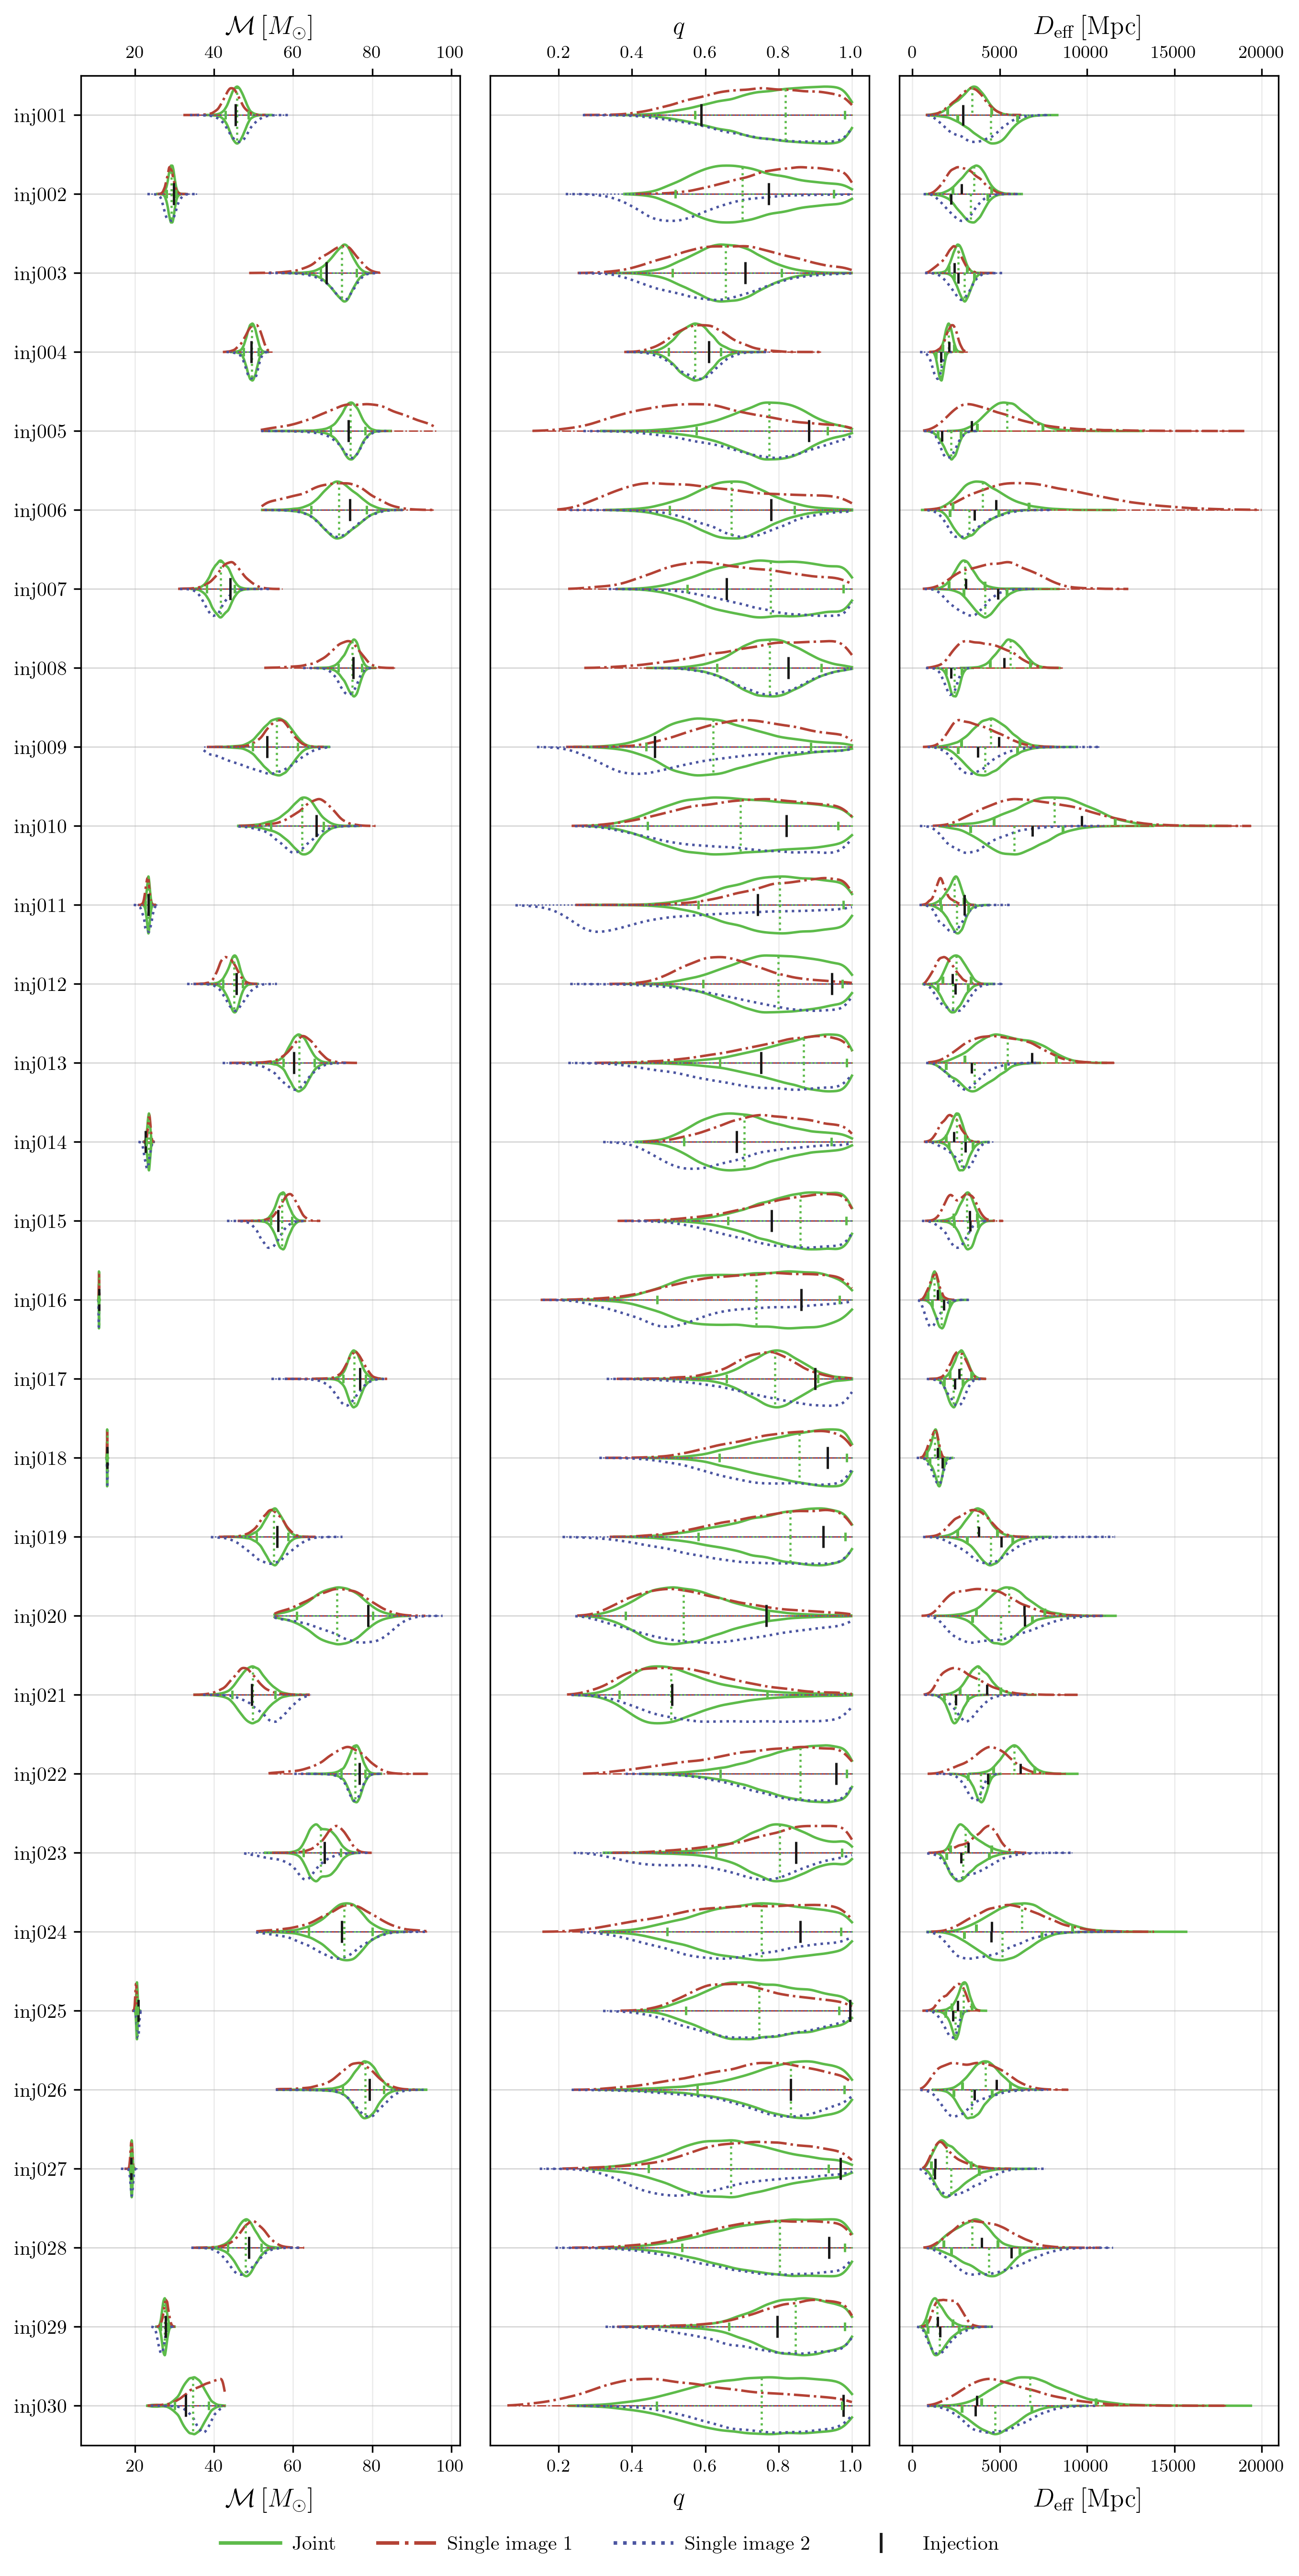
\includegraphics[height=0.92\textheight]{Figures/violin_massdist_p01.png}
    \caption[Posteriors for all events: chirp mass, mass ratio, effective distance]{Recovered posteriors of the chirp mass $\mathcal{M}$, mass ratio $q$, and effective luminosity distance $D_\mathrm{eff}$, for all 150 events (1 of 5). Joint posterior in green (solid), single-image posteriors in red (dash-dot, image 1) and blue (dotted, image 2); the injected value is the black tick.}
    \label{fig:violin_massdist_full}
\end{figure}

\begin{figure}[p]
    \ContinuedFloat
    \centering
    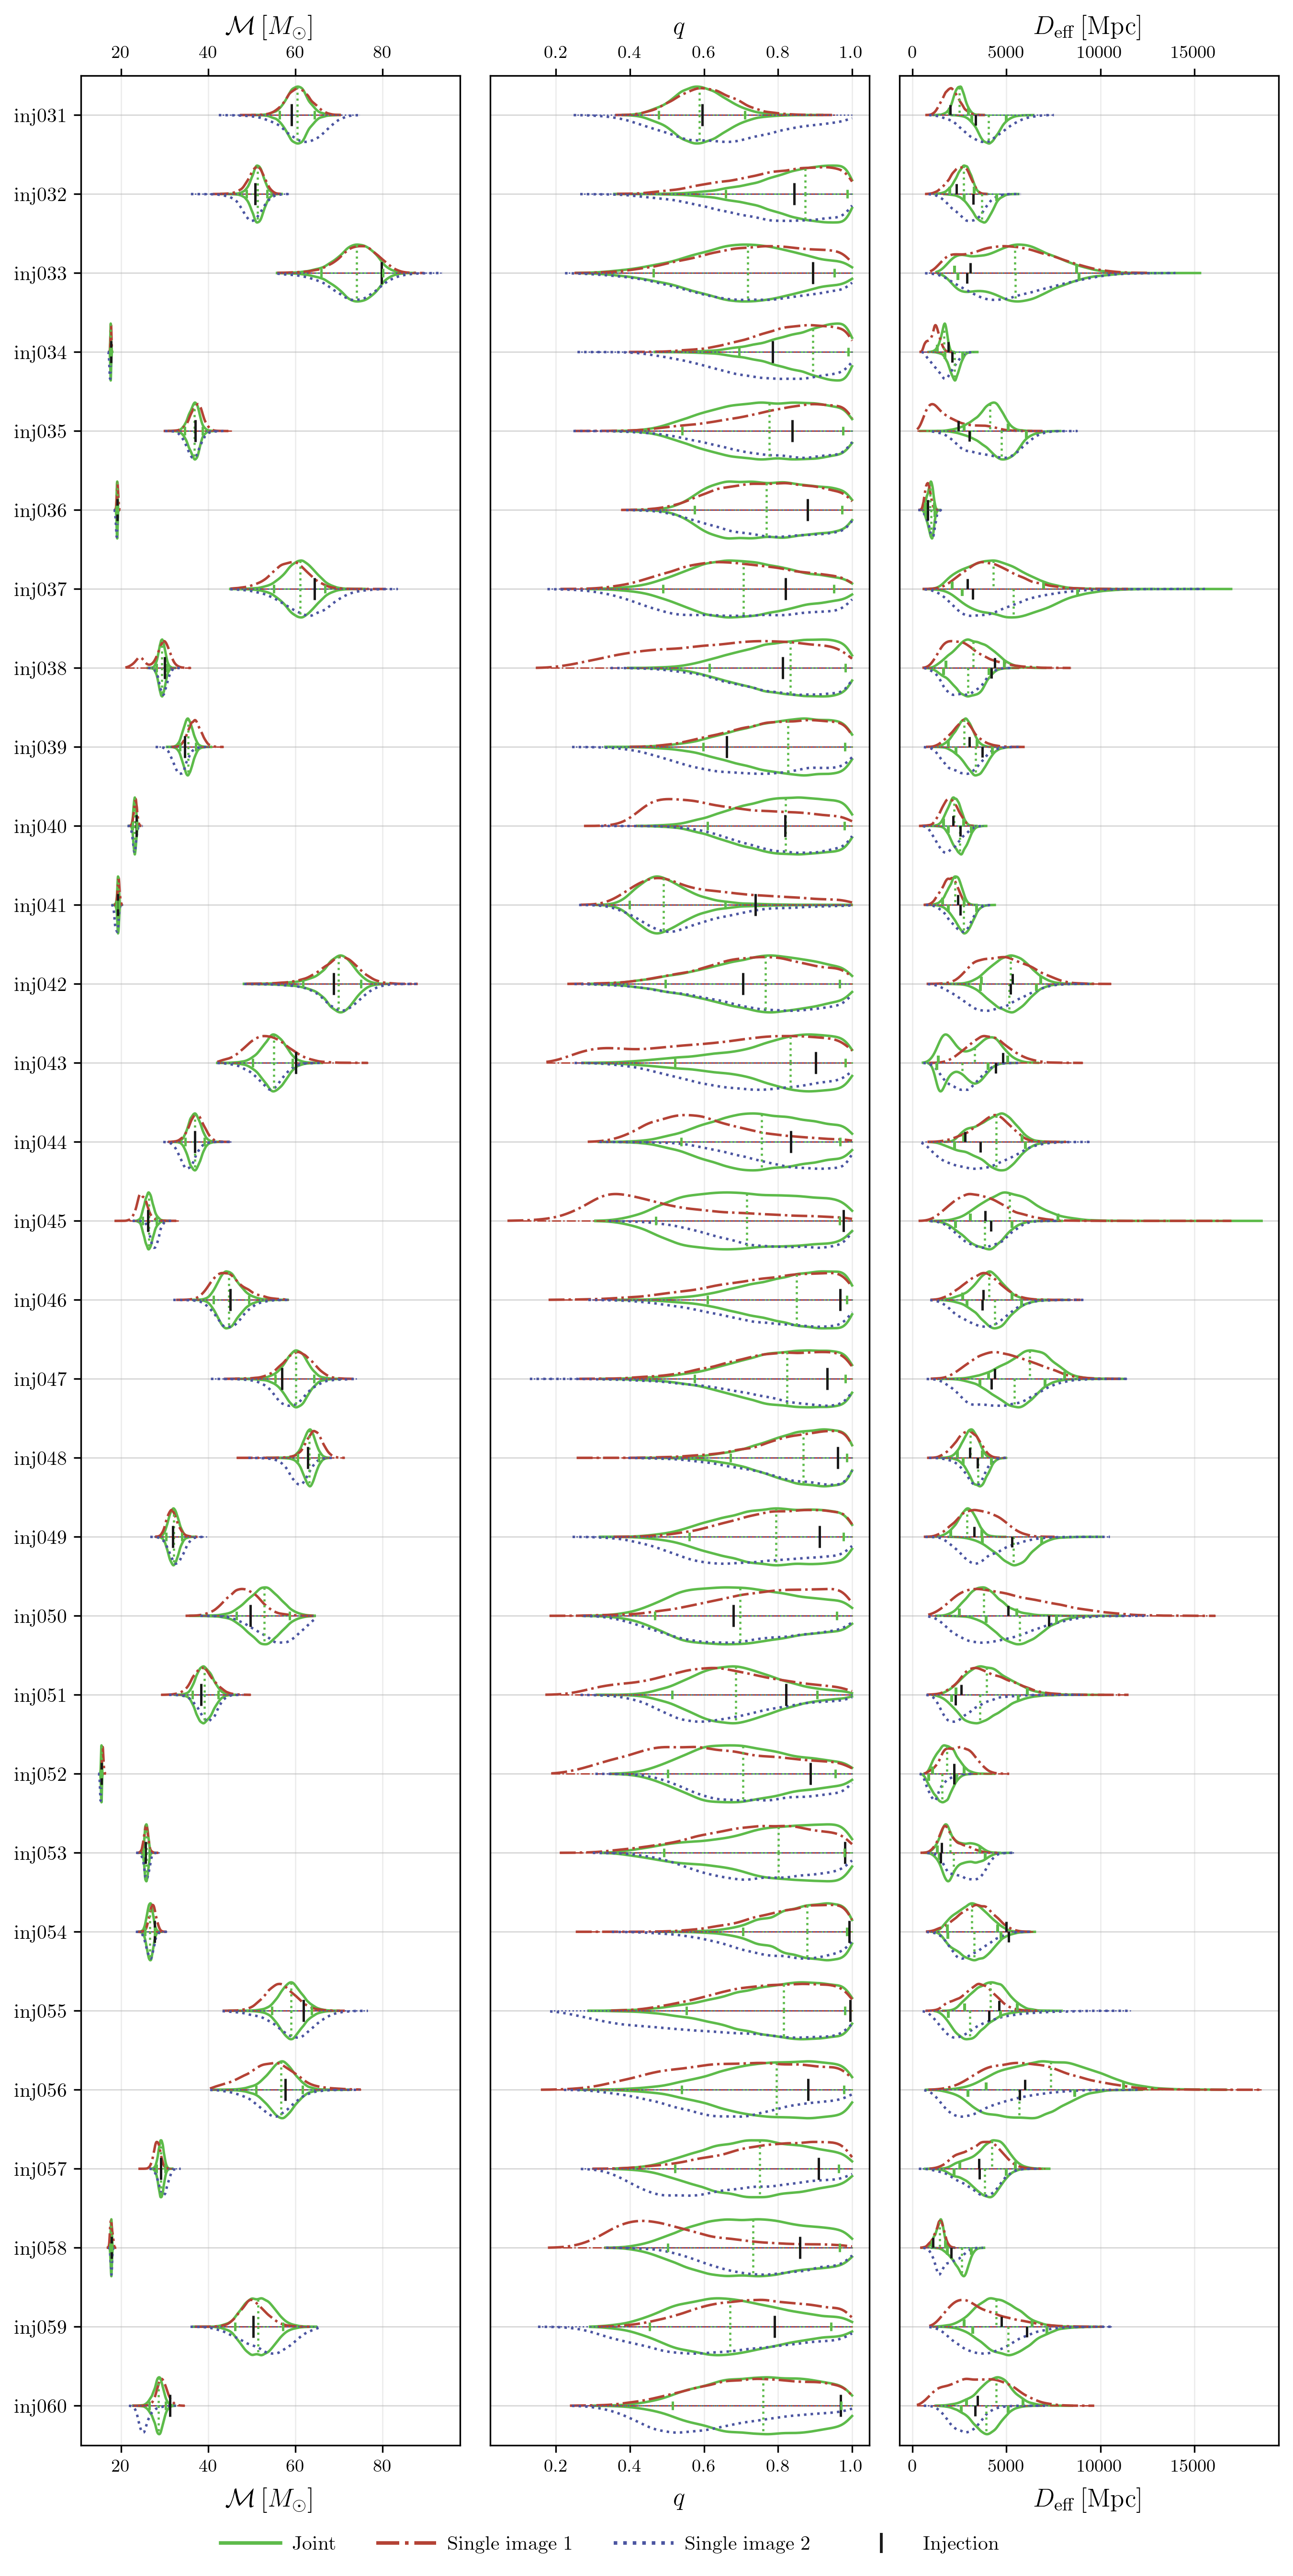
\includegraphics[height=0.92\textheight]{Figures/violin_massdist_p02.png}
    \caption[]{Recovered posteriors of $\mathcal{M}$, $q$, and $D_\mathrm{eff}$ (2 of 5).}
\end{figure}

\begin{figure}[p]
    \ContinuedFloat
    \centering
    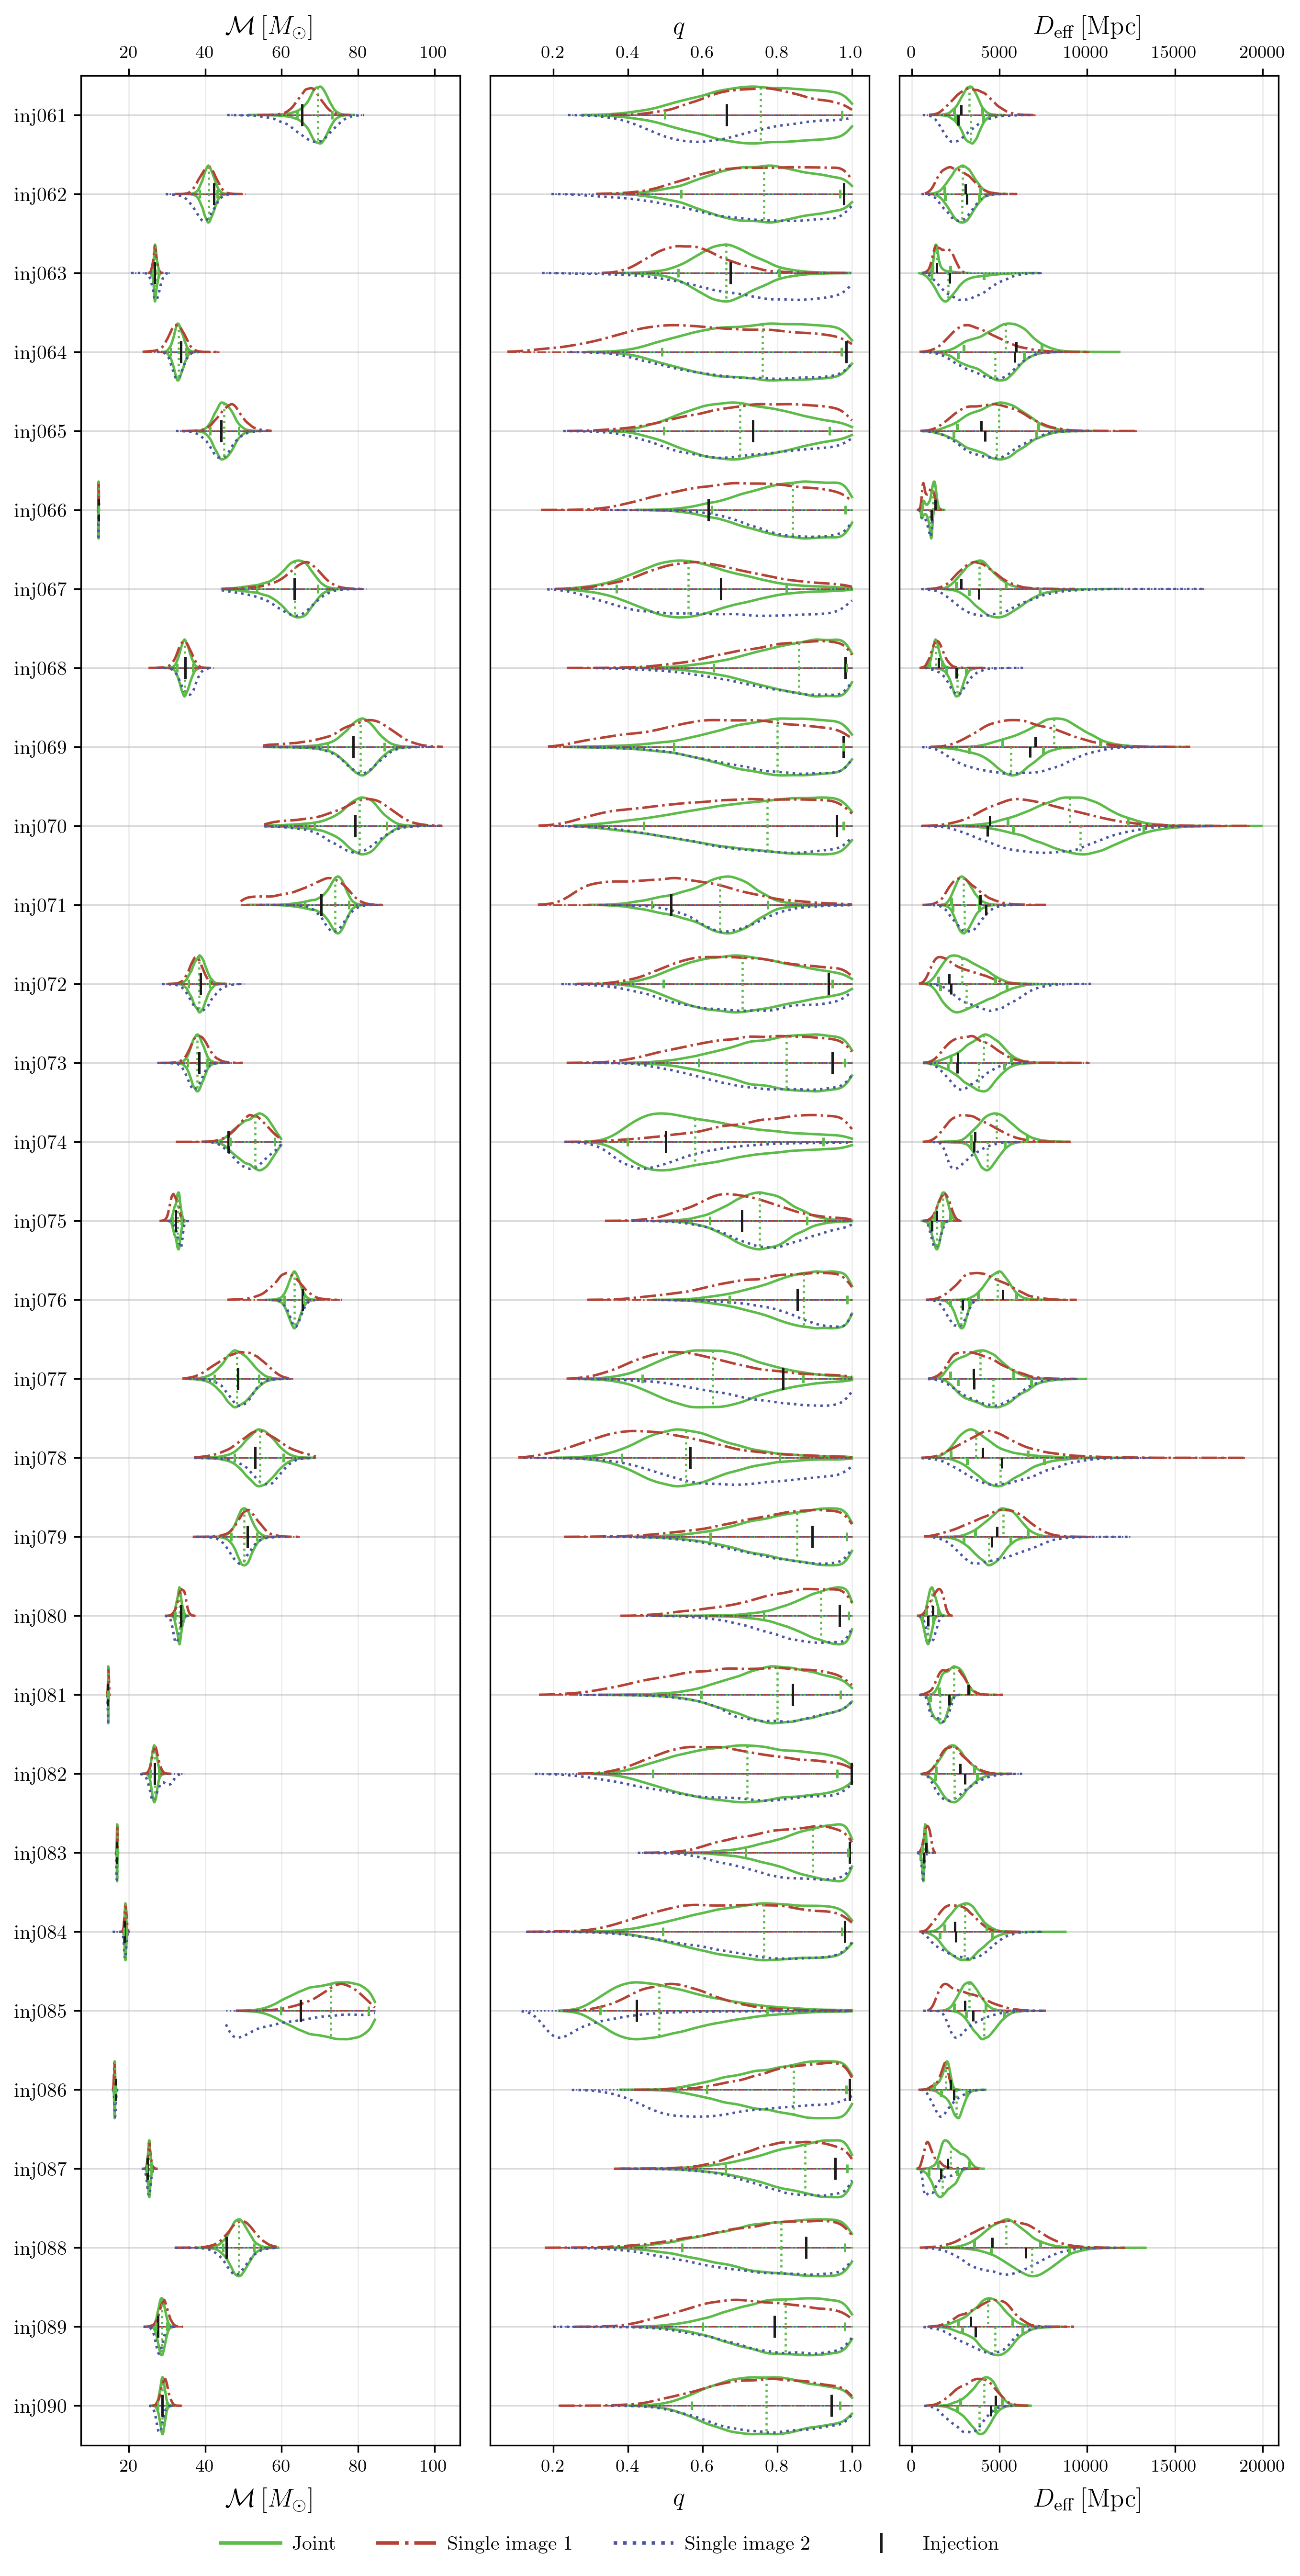
\includegraphics[height=0.92\textheight]{Figures/violin_massdist_p03.png}
    \caption[]{Recovered posteriors of $\mathcal{M}$, $q$, and $D_\mathrm{eff}$ (3 of 5).}
\end{figure}

\begin{figure}[p]
    \ContinuedFloat
    \centering
    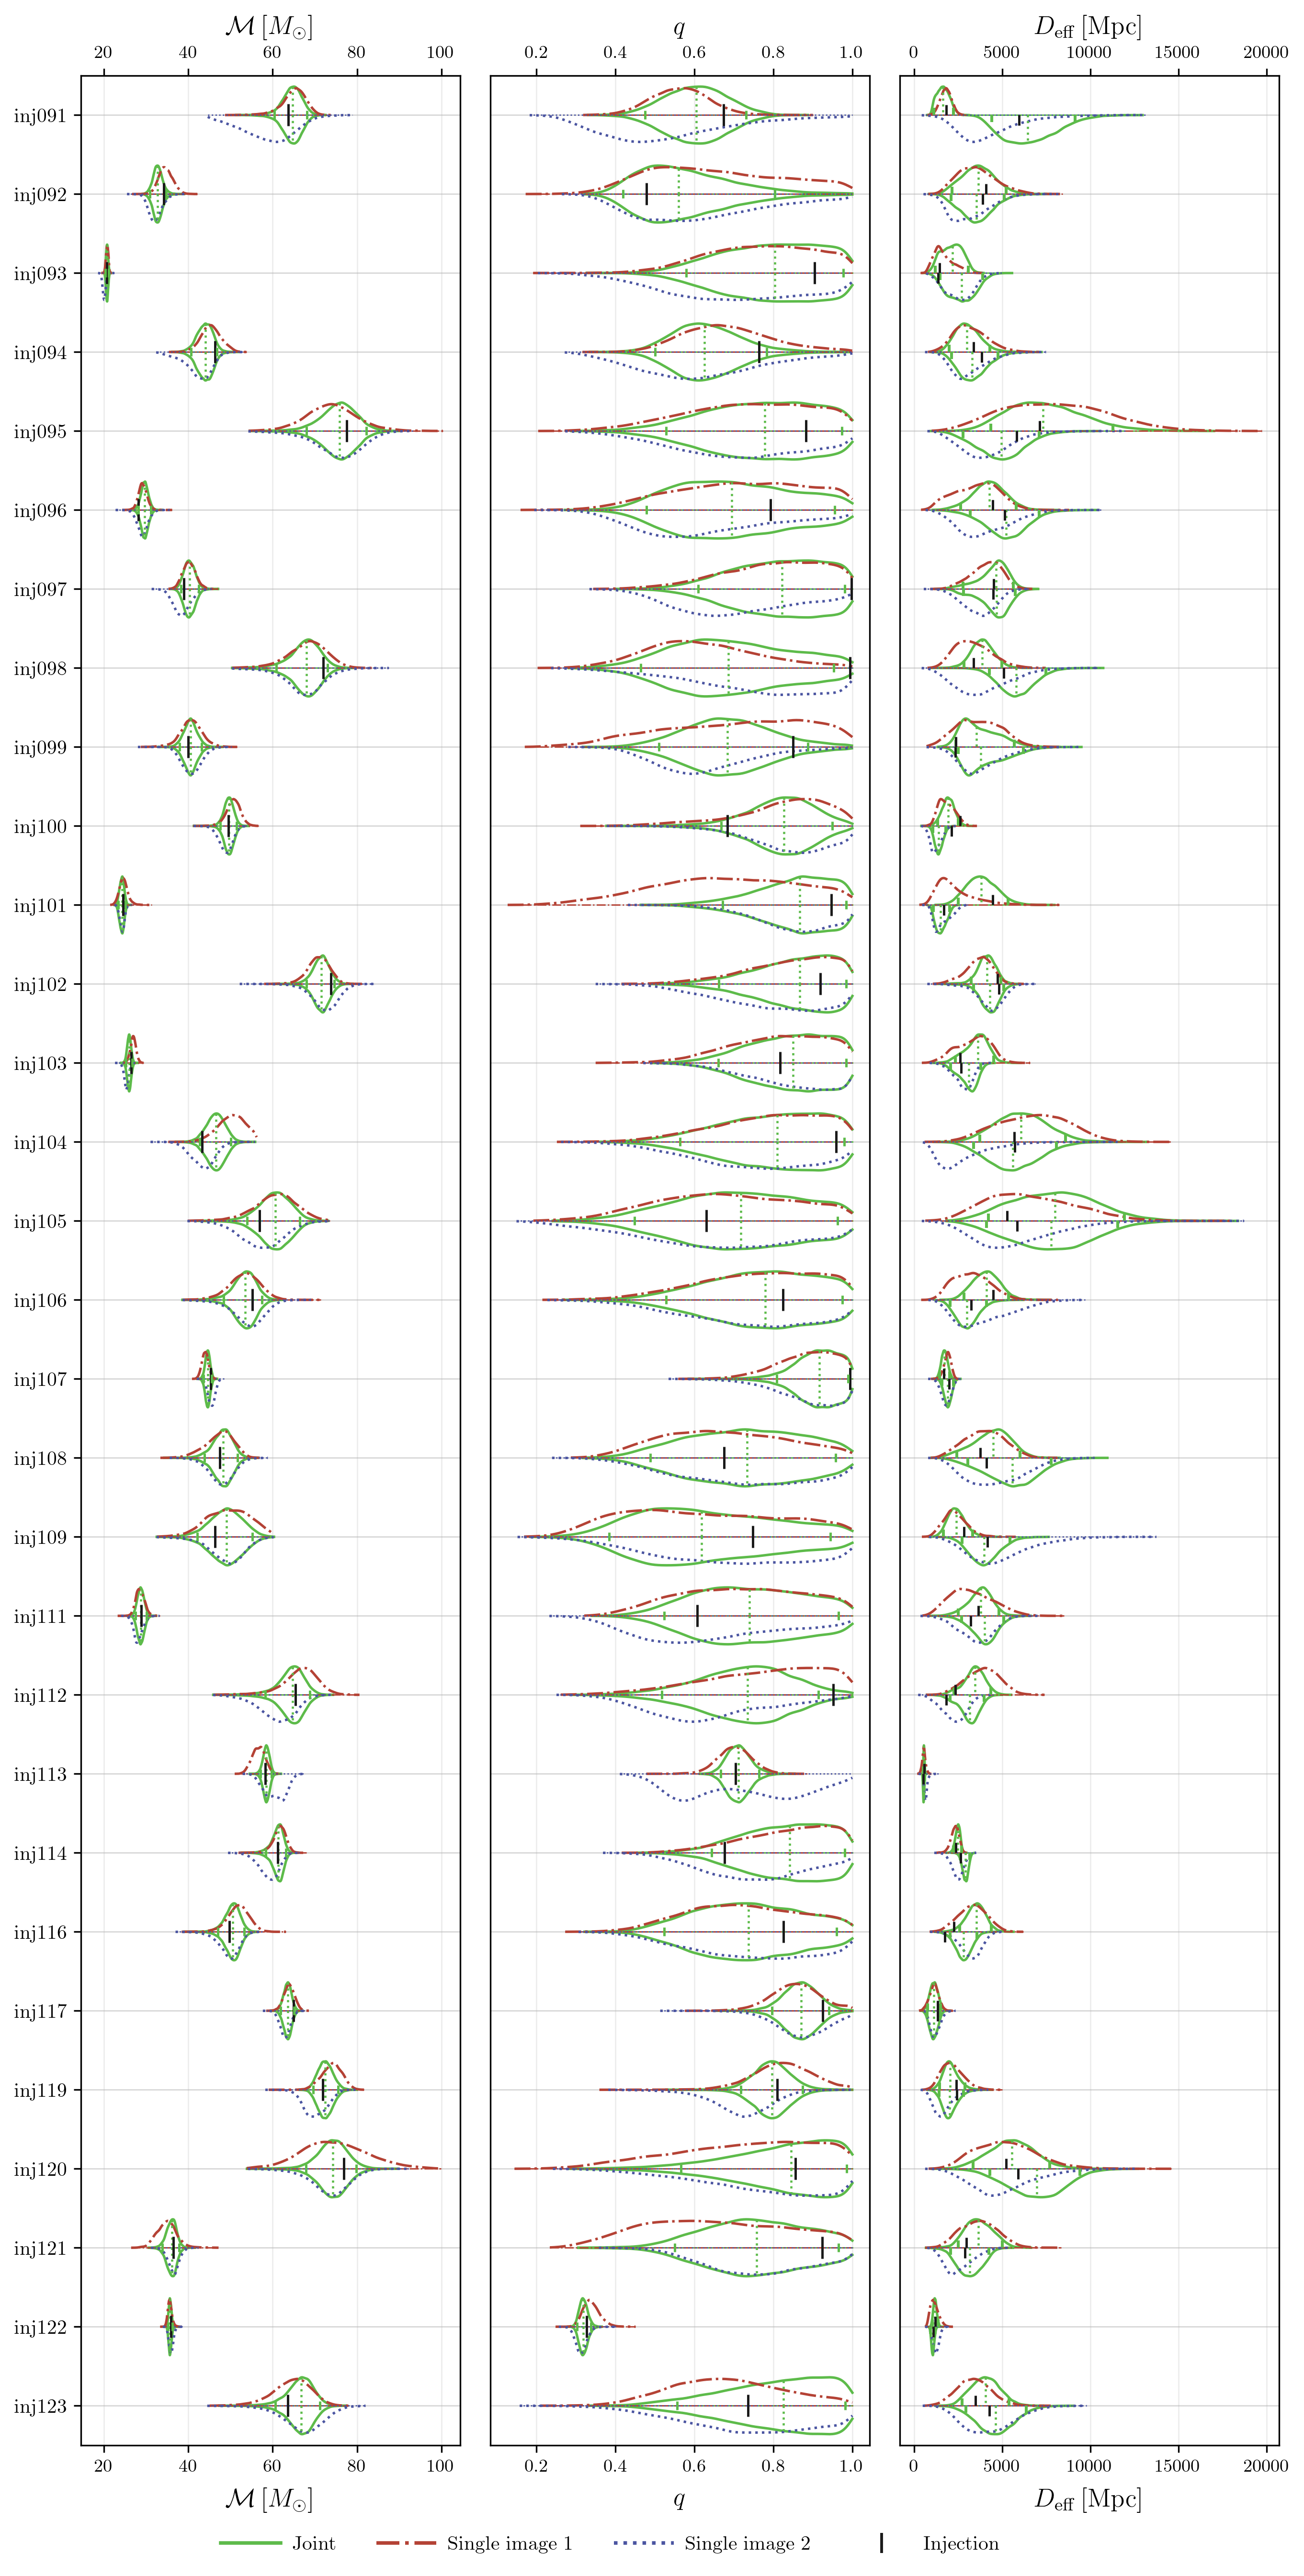
\includegraphics[height=0.92\textheight]{Figures/violin_massdist_p04.png}
    \caption[]{Recovered posteriors of $\mathcal{M}$, $q$, and $D_\mathrm{eff}$ (4 of 5).}
\end{figure}

\begin{figure}[p]
    \ContinuedFloat
    \centering
    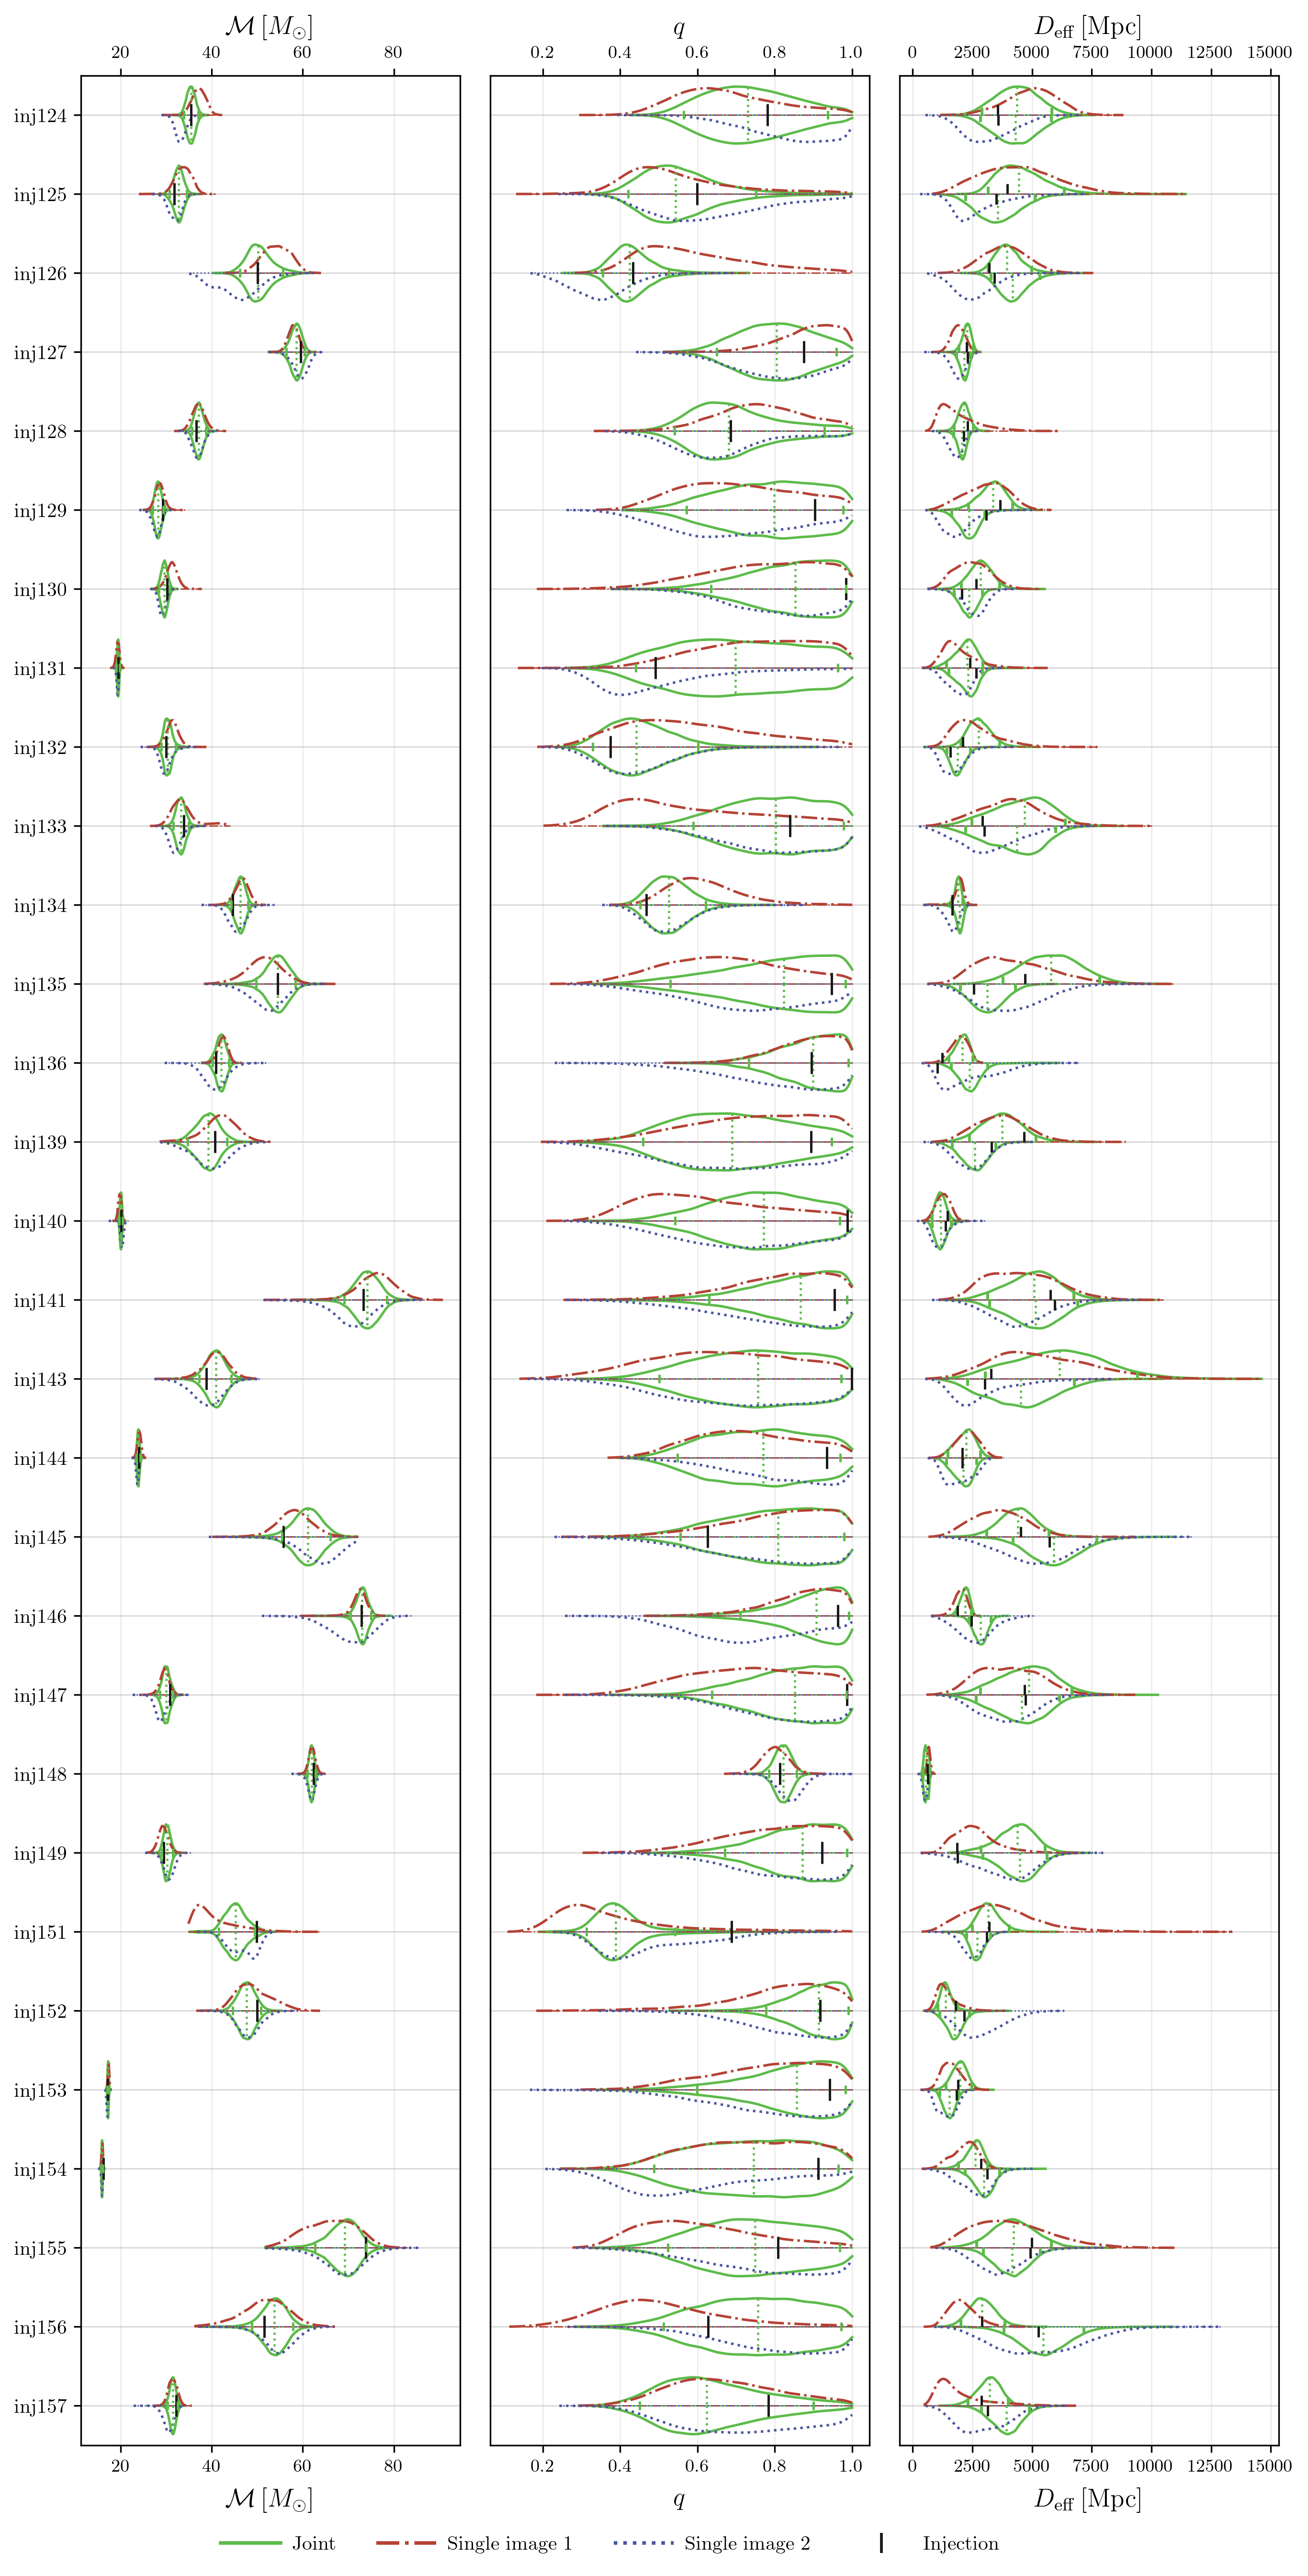
\includegraphics[height=0.92\textheight]{Figures/violin_massdist_p05.png}
    \caption[]{Recovered posteriors of $\mathcal{M}$, $q$, and $D_\mathrm{eff}$ (5 of 5).}
\end{figure}


% Set B: spin parameters

\begin{figure}[p]
    \centering
    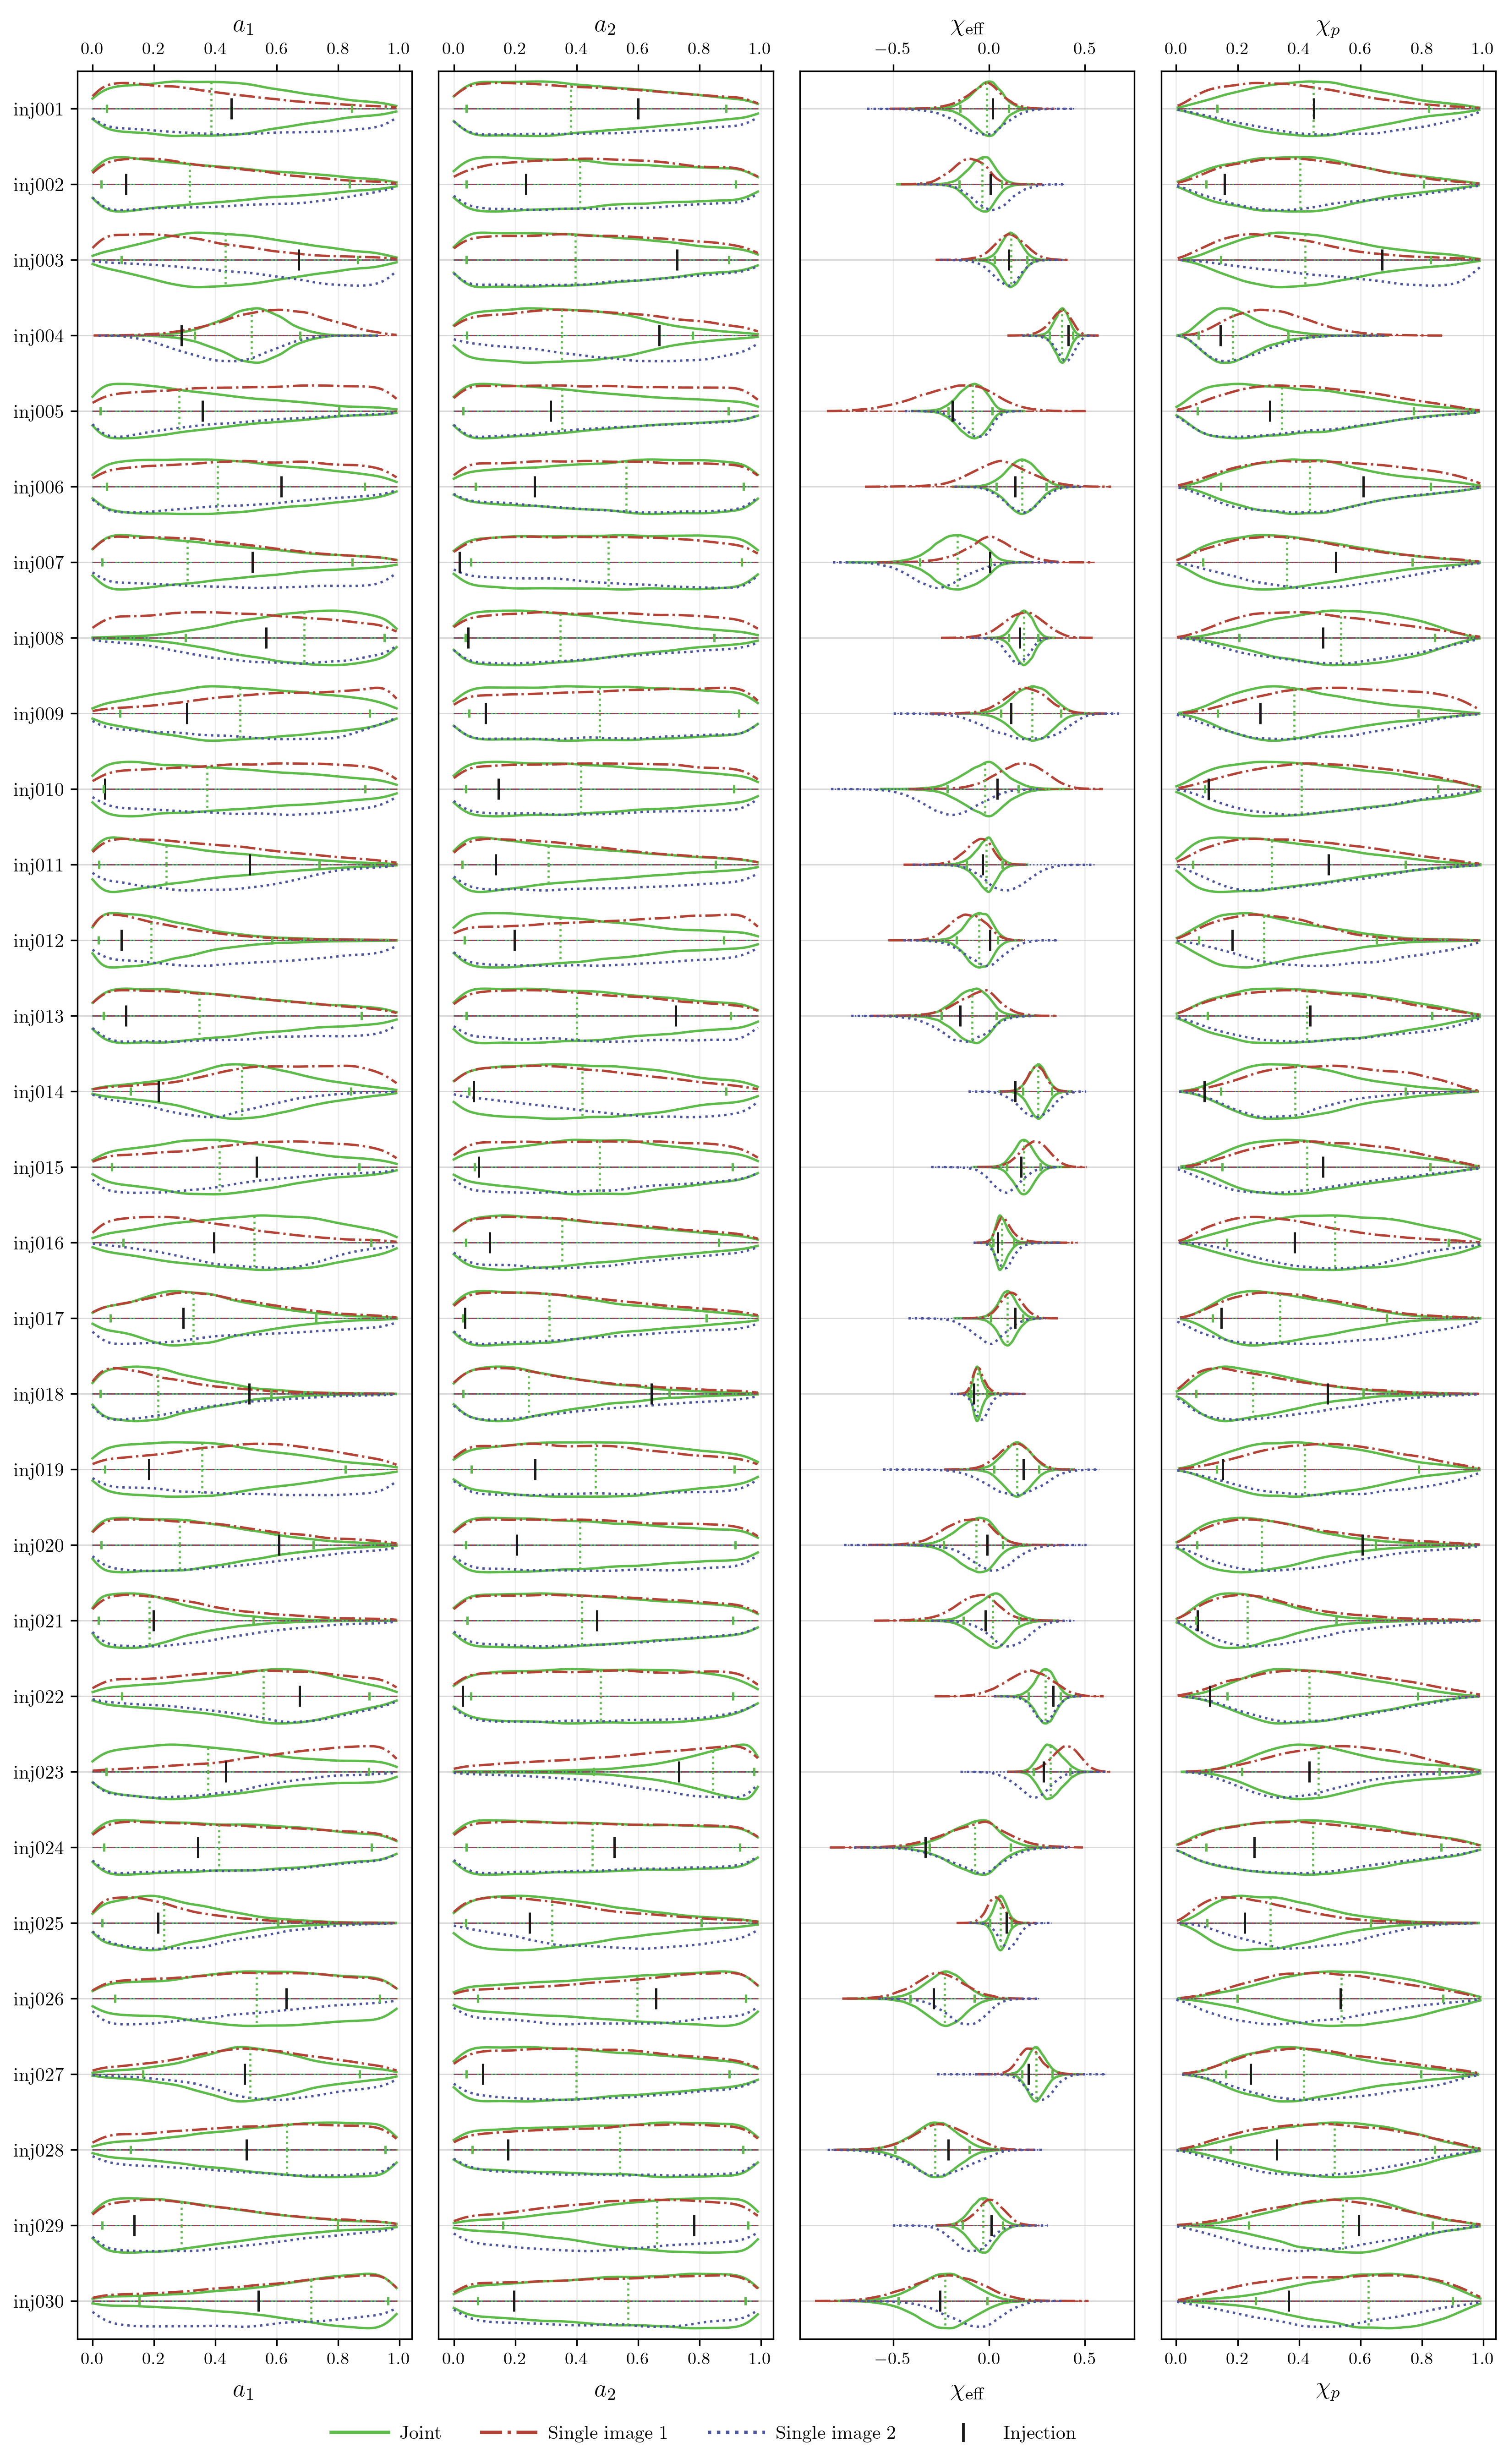
\includegraphics[height=0.92\textheight]{Figures/violin_spins_p01.png}
    \caption[Posteriors for all events: spin parameters]{Recovered posteriors of the spin magnitudes $a_1$ and $a_2$, effective spin $\chi_\mathrm{eff}$, and precessing spin $\chi_\mathrm{p}$, for all 150 events (1 of 5). Colors as in Figure~\ref{fig:violin_massdist_full}.}
    \label{fig:violin_spins_full}
\end{figure}

\begin{figure}[p]
    \ContinuedFloat
    \centering
    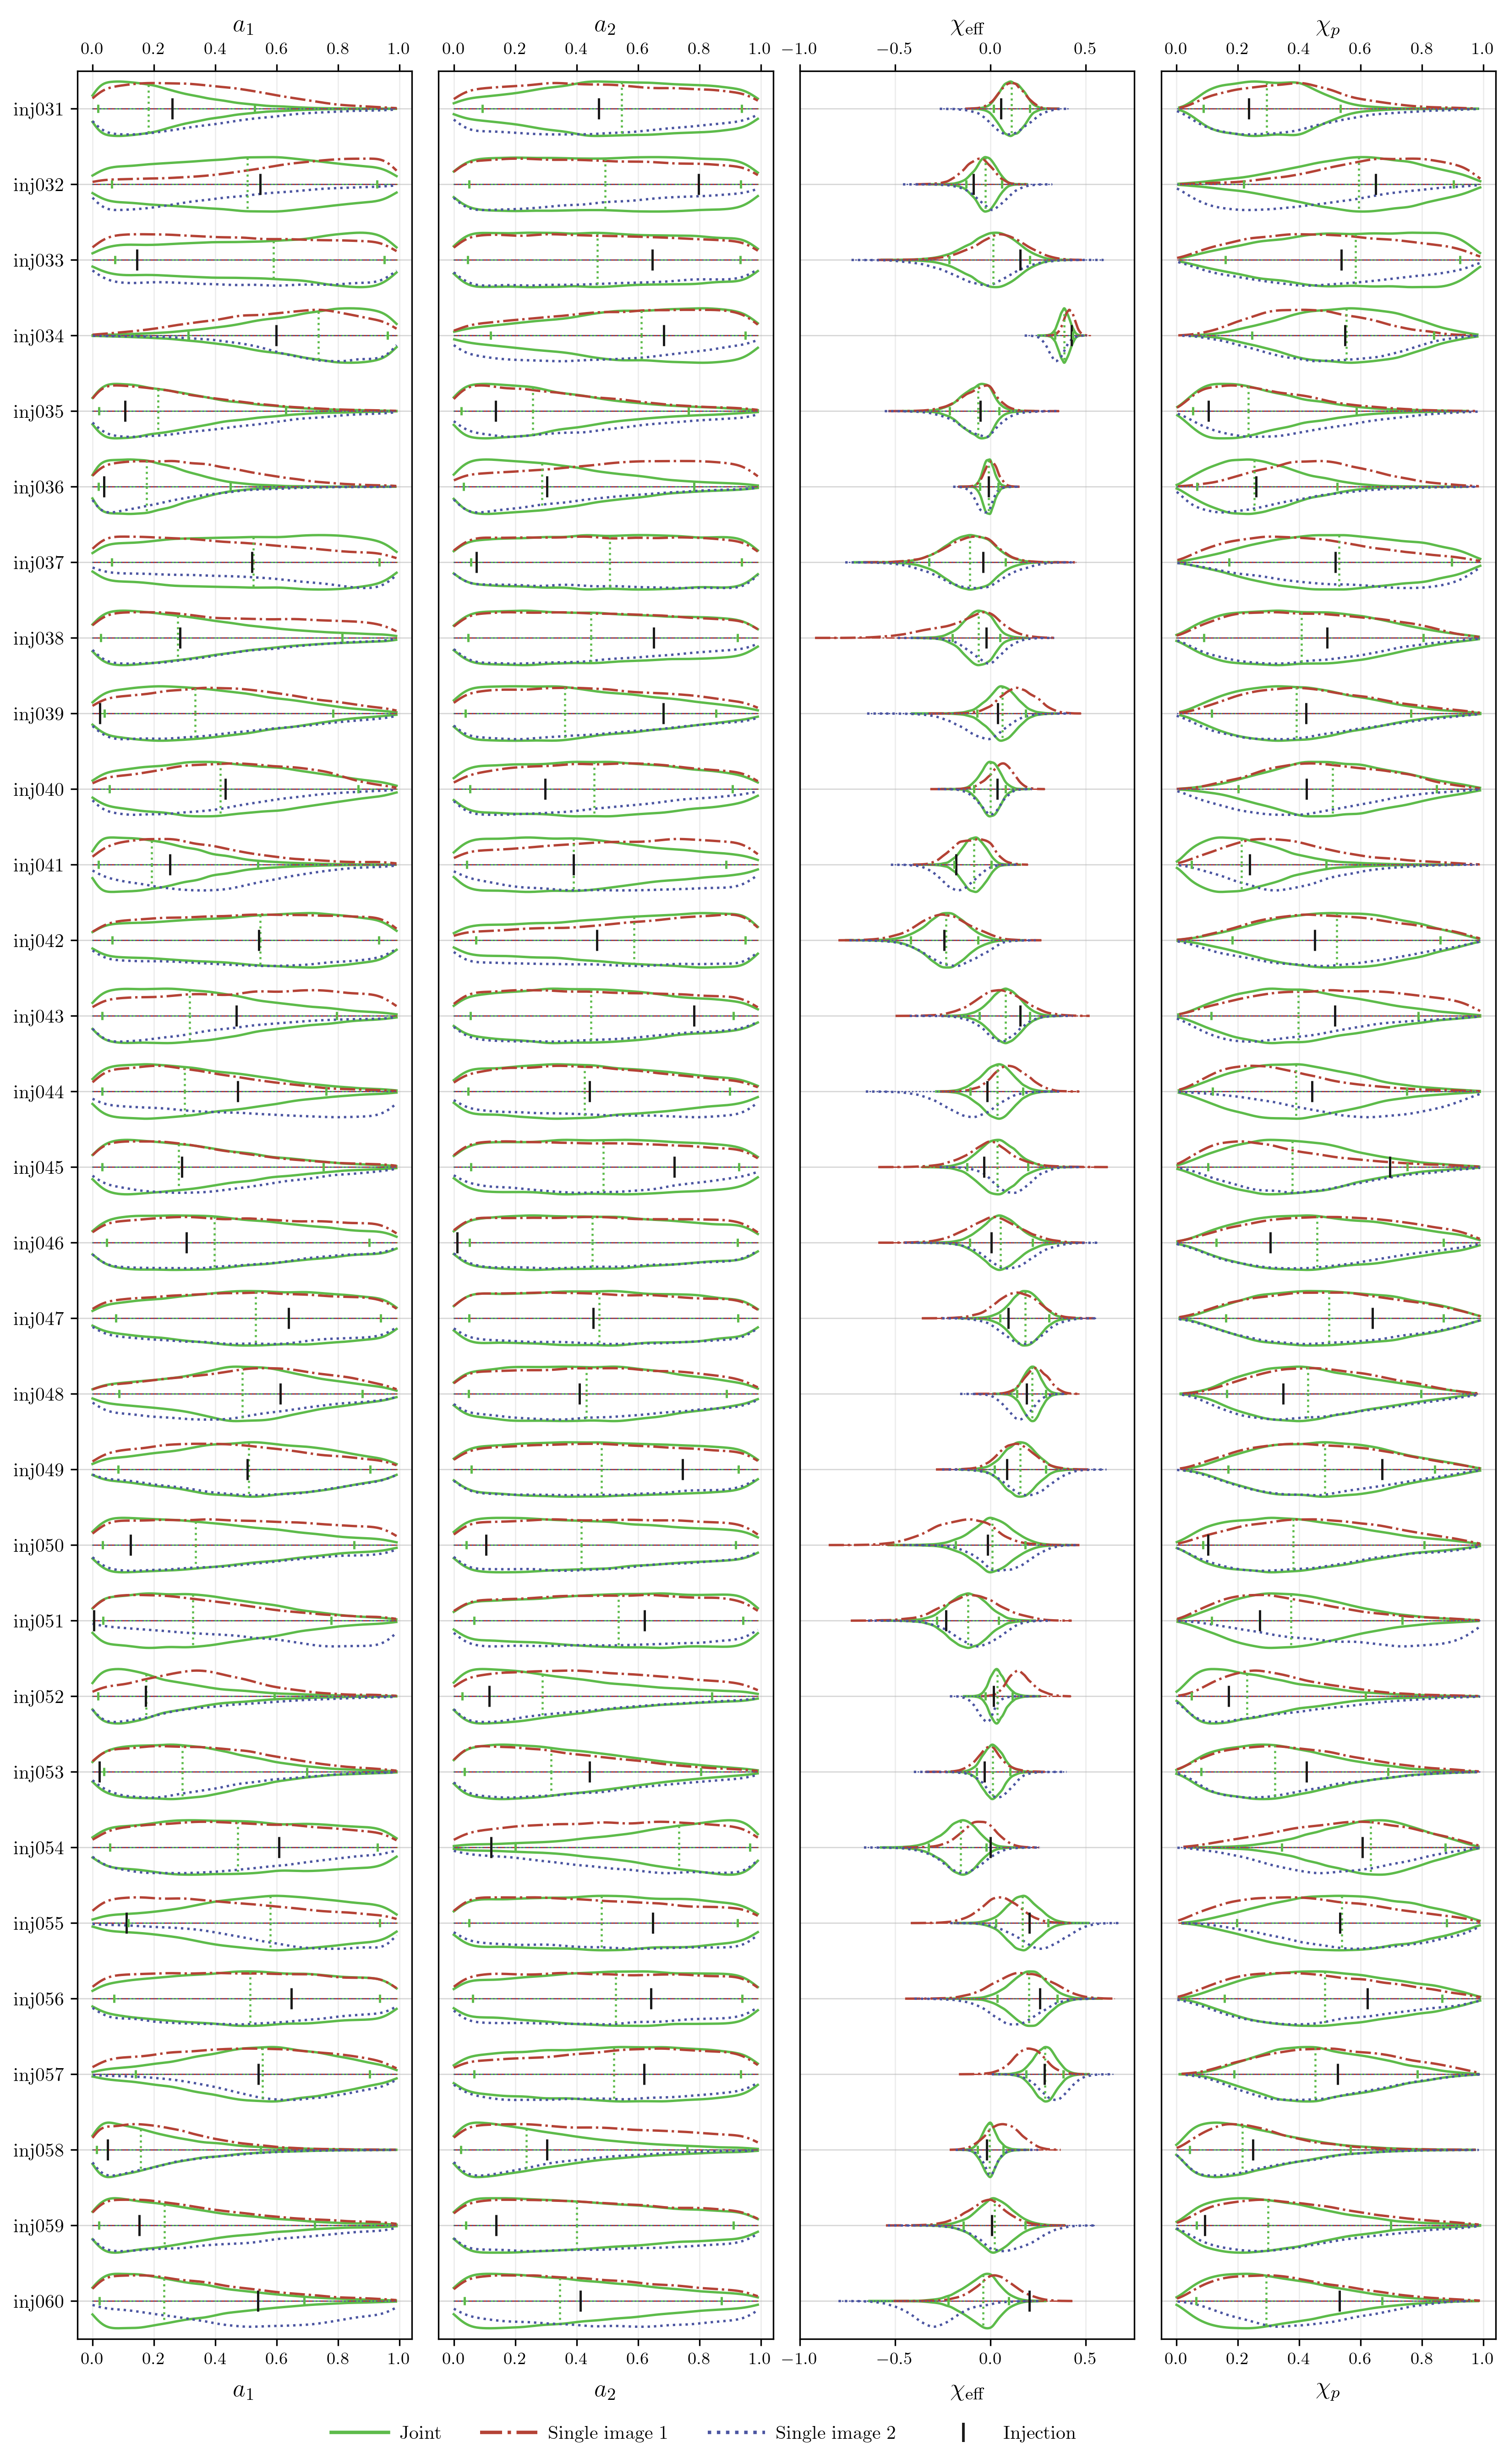
\includegraphics[height=0.92\textheight]{Figures/violin_spins_p02.png}
    \caption[]{Recovered posteriors of $a_1$, $a_2$, $\chi_\mathrm{eff}$, and $\chi_\mathrm{p}$ (2 of 5).}
\end{figure}

\begin{figure}[p]
    \ContinuedFloat
    \centering
    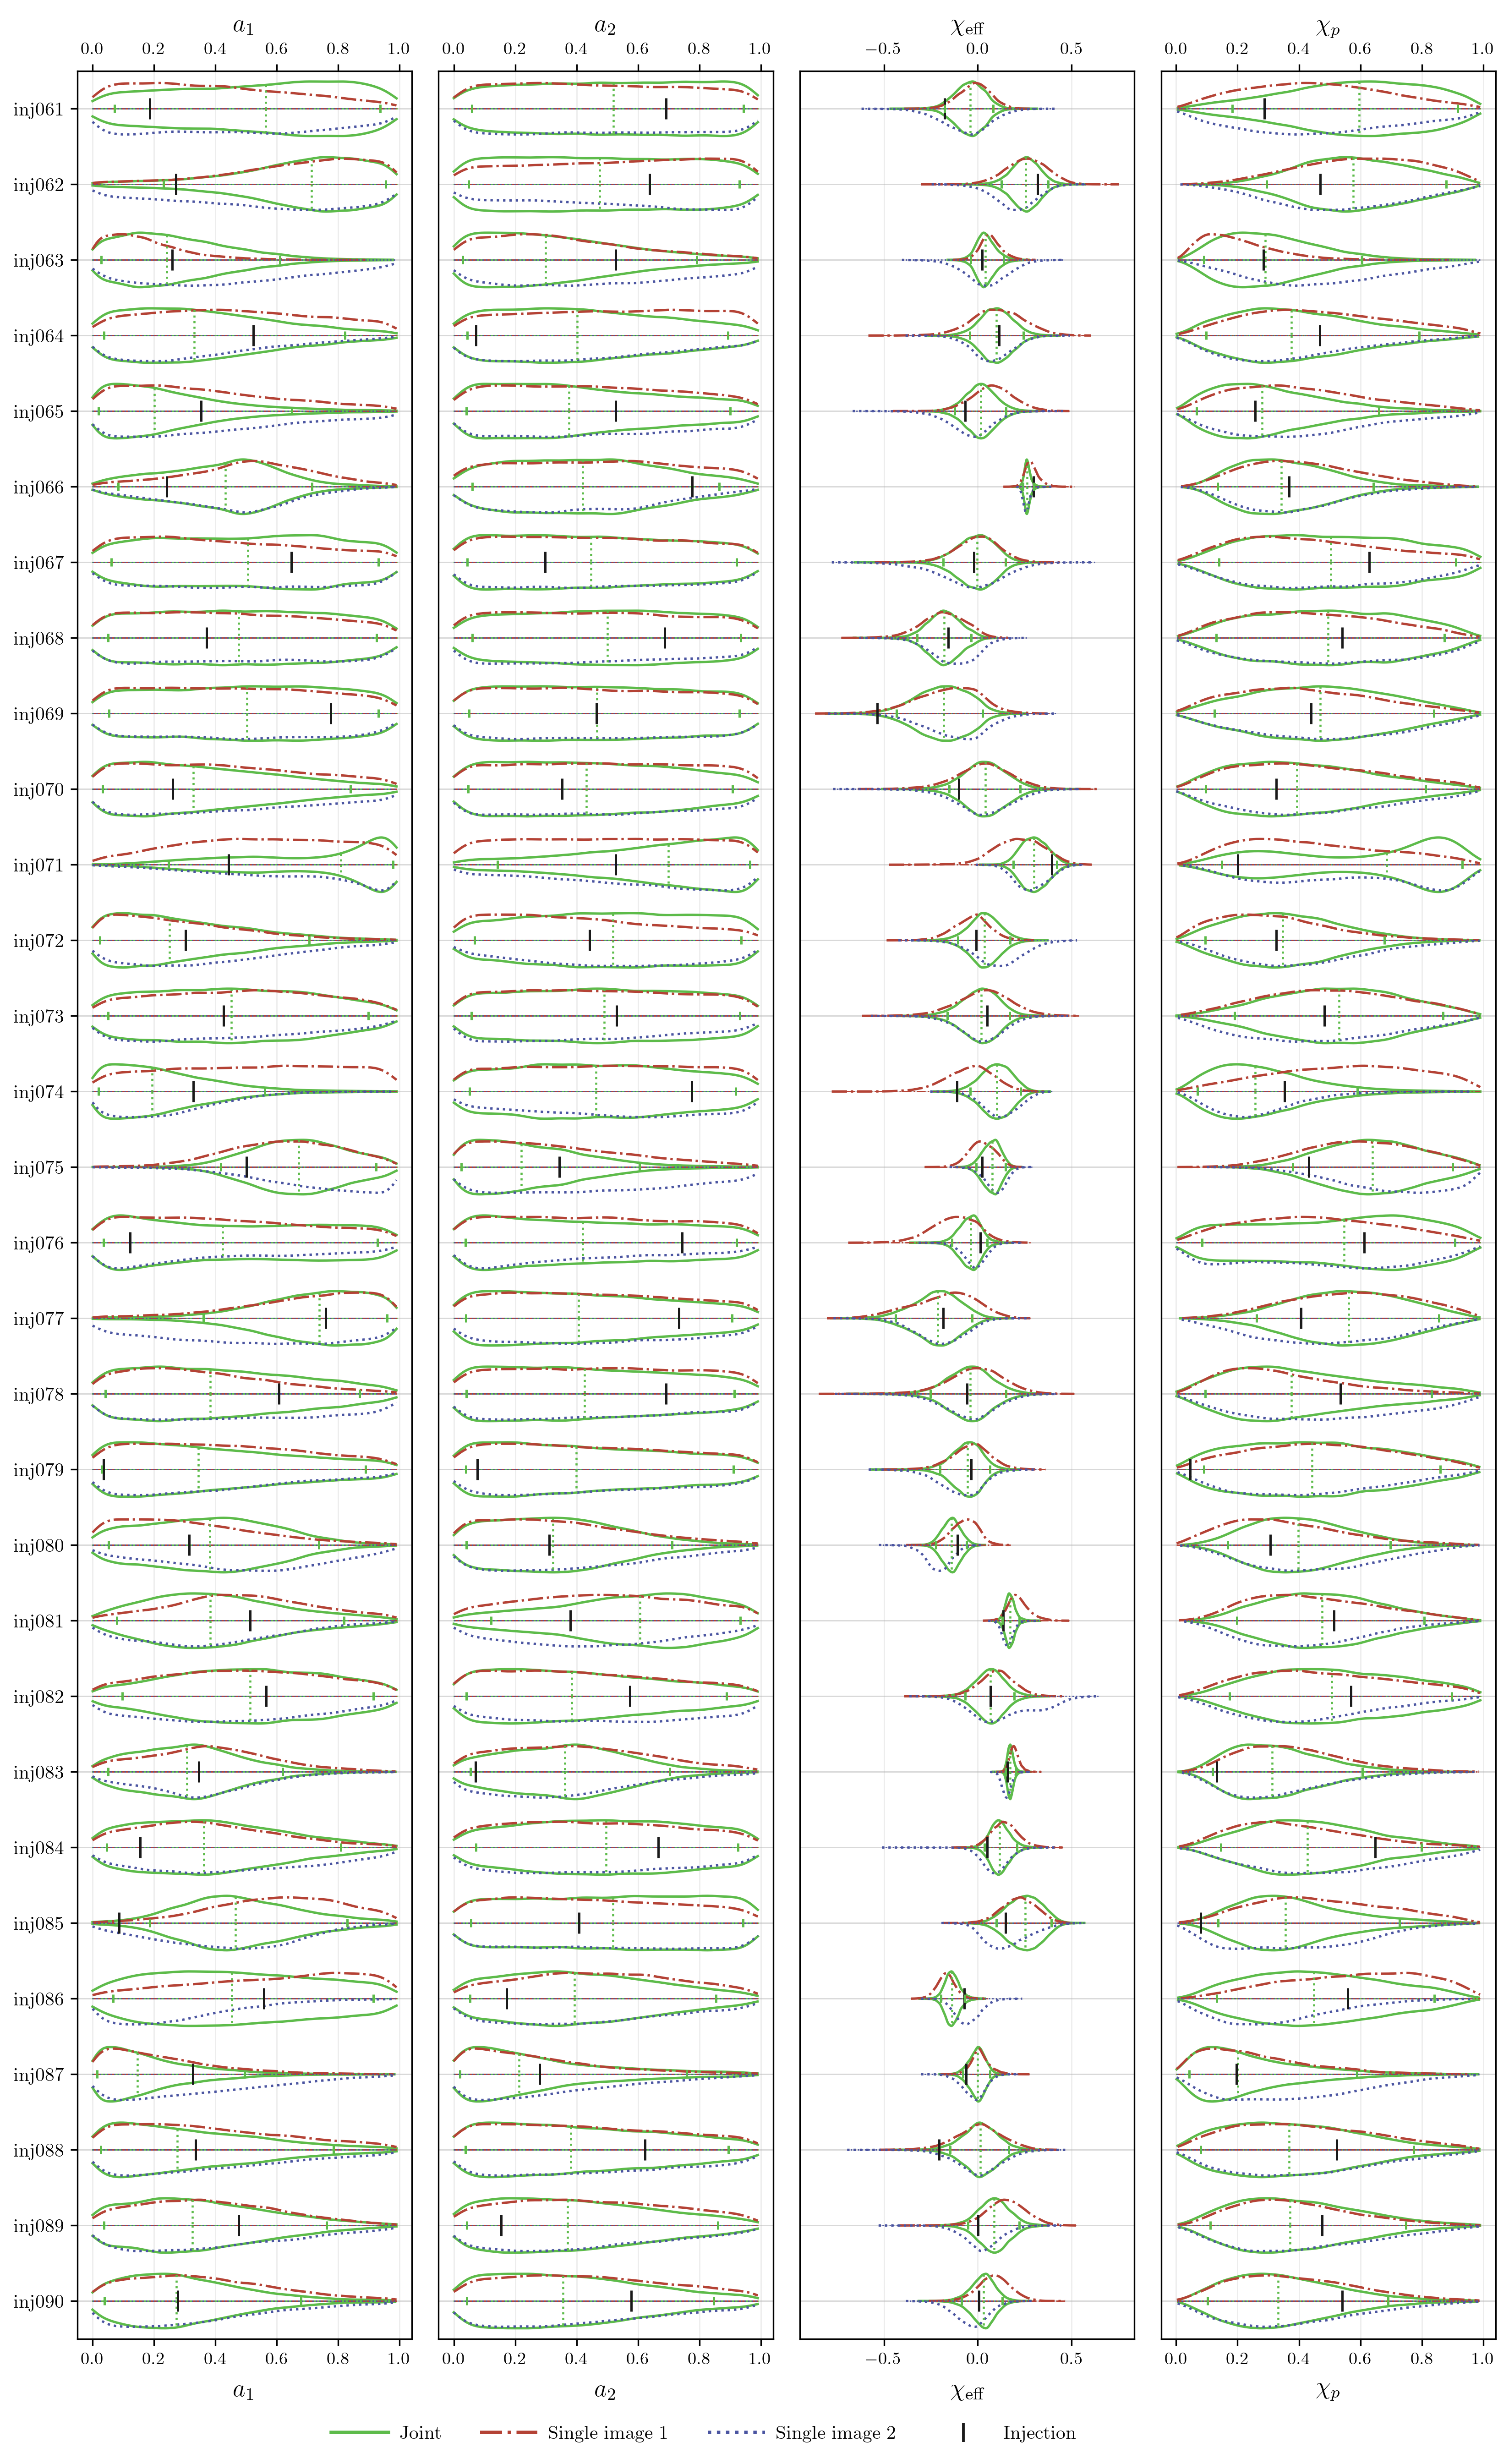
\includegraphics[height=0.92\textheight]{Figures/violin_spins_p03.png}
    \caption[]{Recovered posteriors of $a_1$, $a_2$, $\chi_\mathrm{eff}$, and $\chi_\mathrm{p}$ (3 of 5).}
\end{figure}

\begin{figure}[p]
    \ContinuedFloat
    \centering
    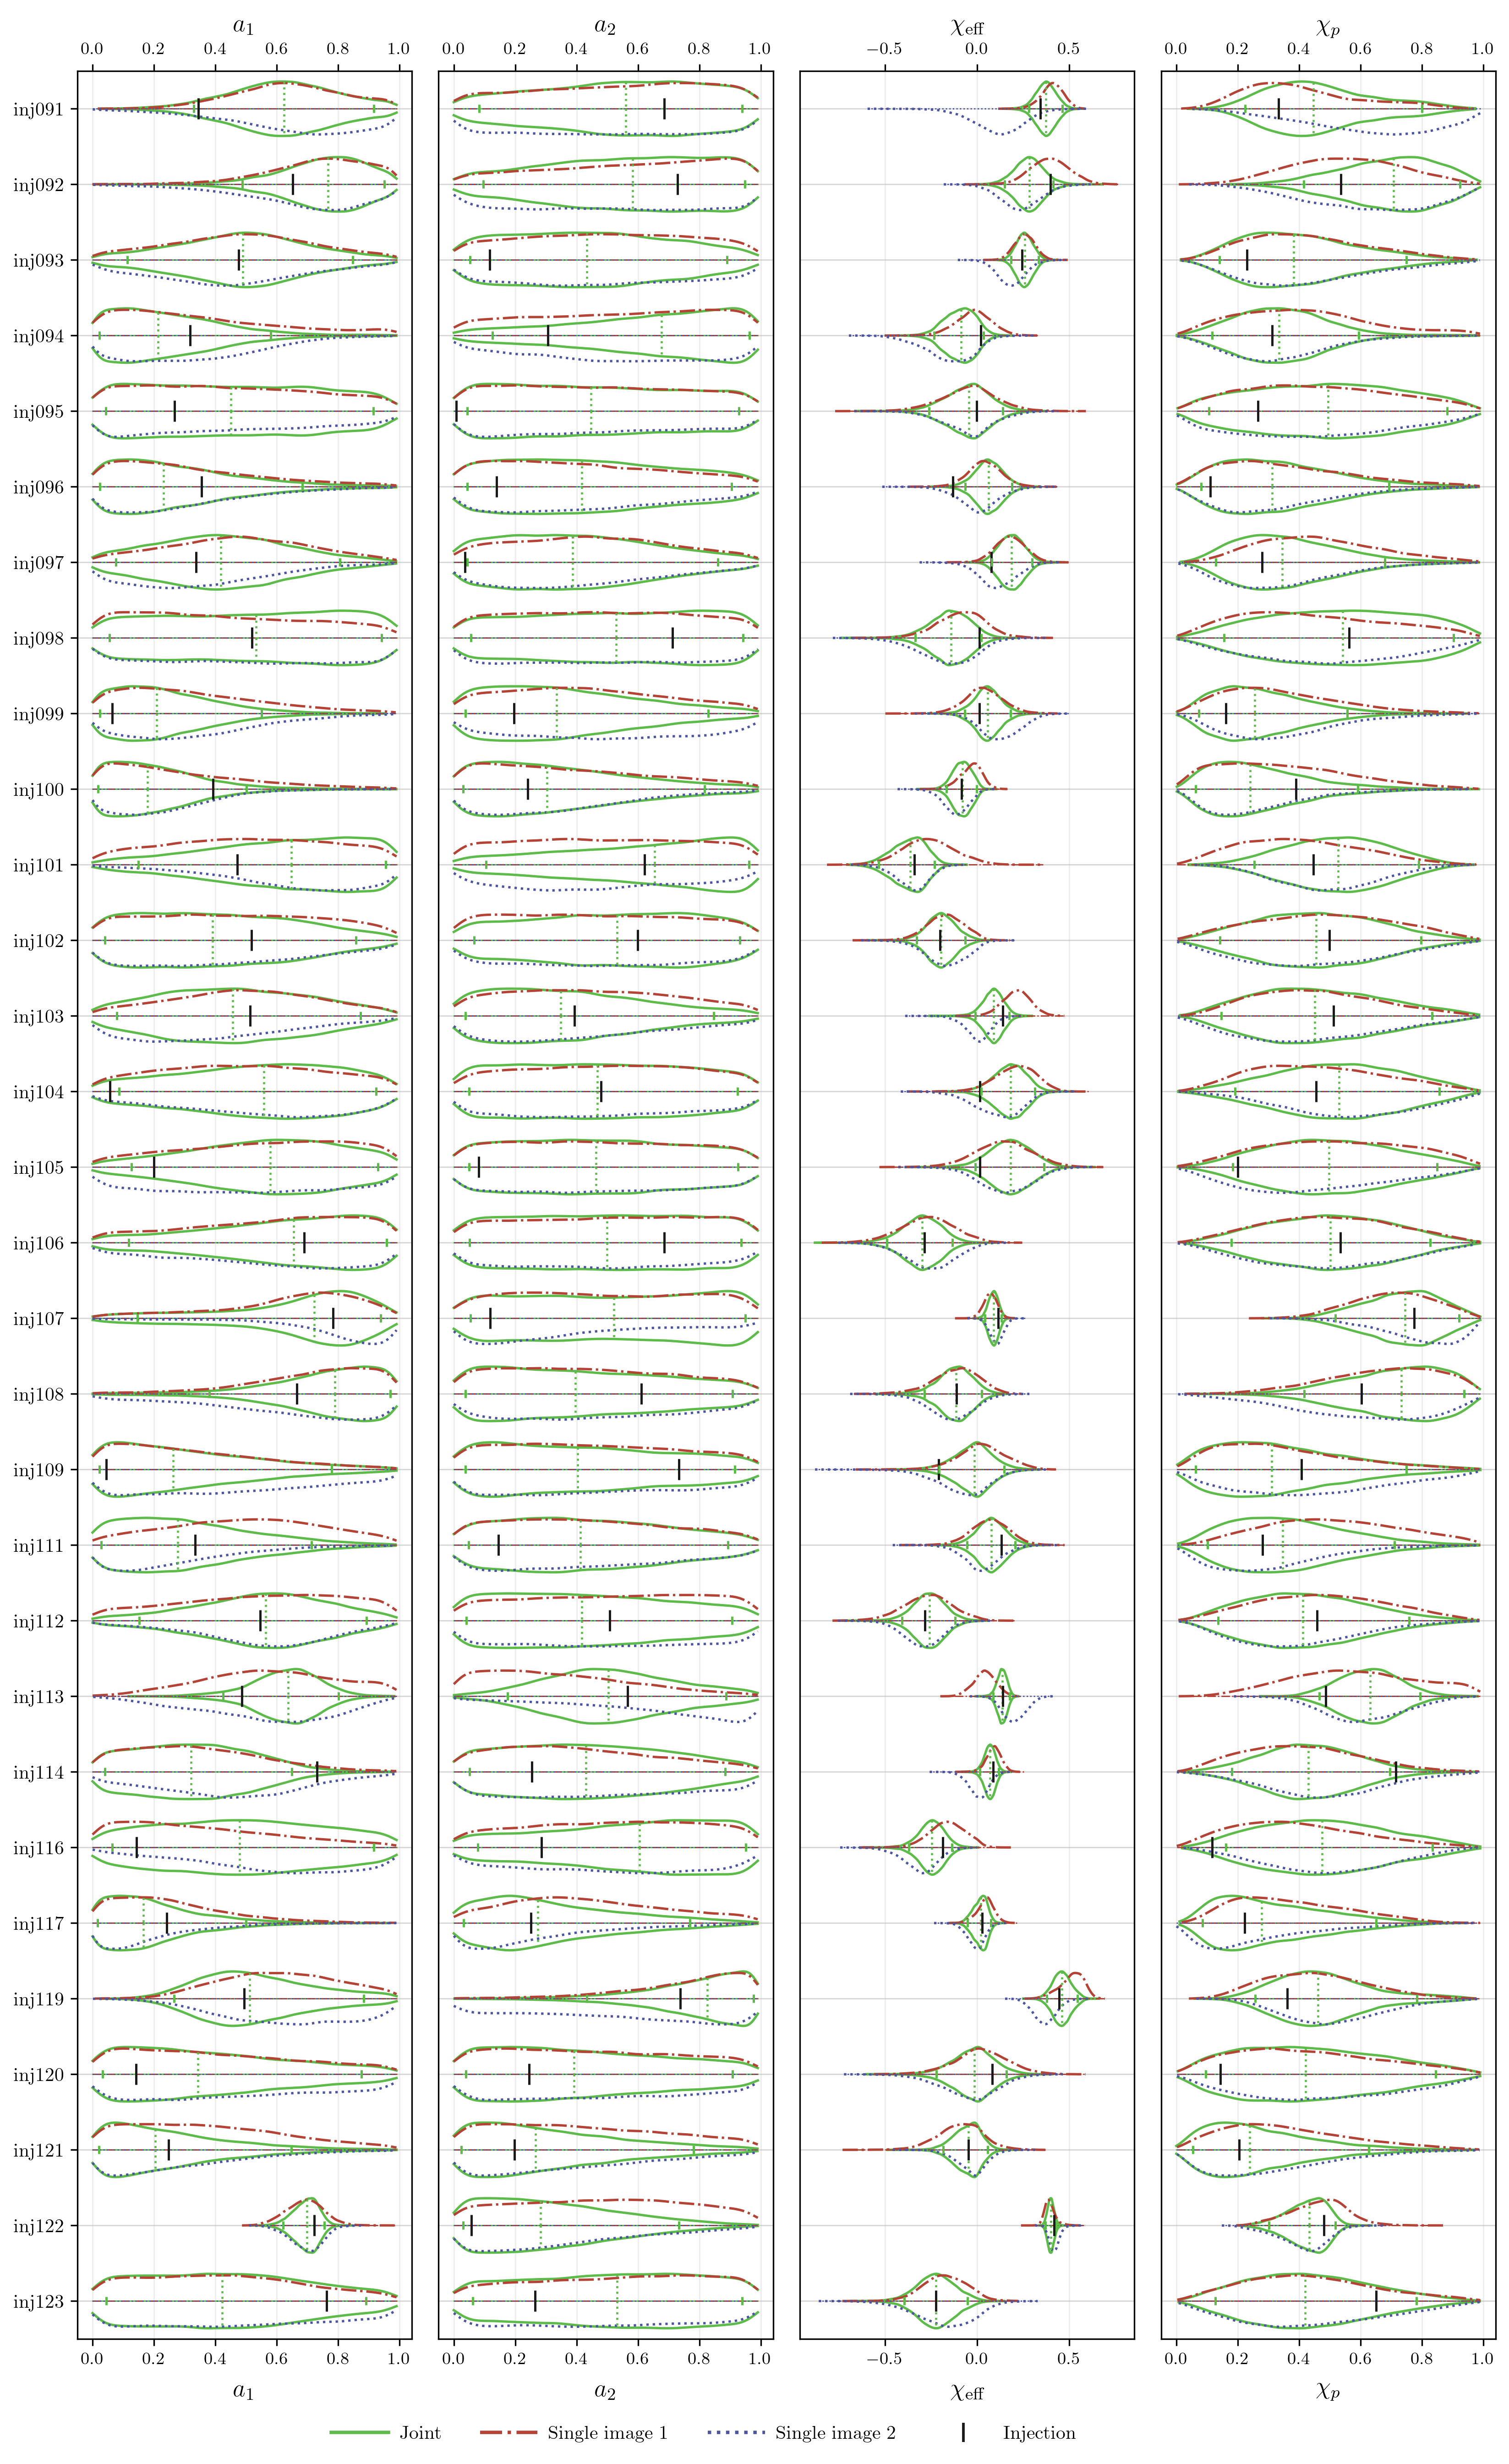
\includegraphics[height=0.92\textheight]{Figures/violin_spins_p04.png}
    \caption[]{Recovered posteriors of $a_1$, $a_2$, $\chi_\mathrm{eff}$, and $\chi_\mathrm{p}$ (4 of 5).}
\end{figure}

\begin{figure}[p]
    \ContinuedFloat
    \centering
    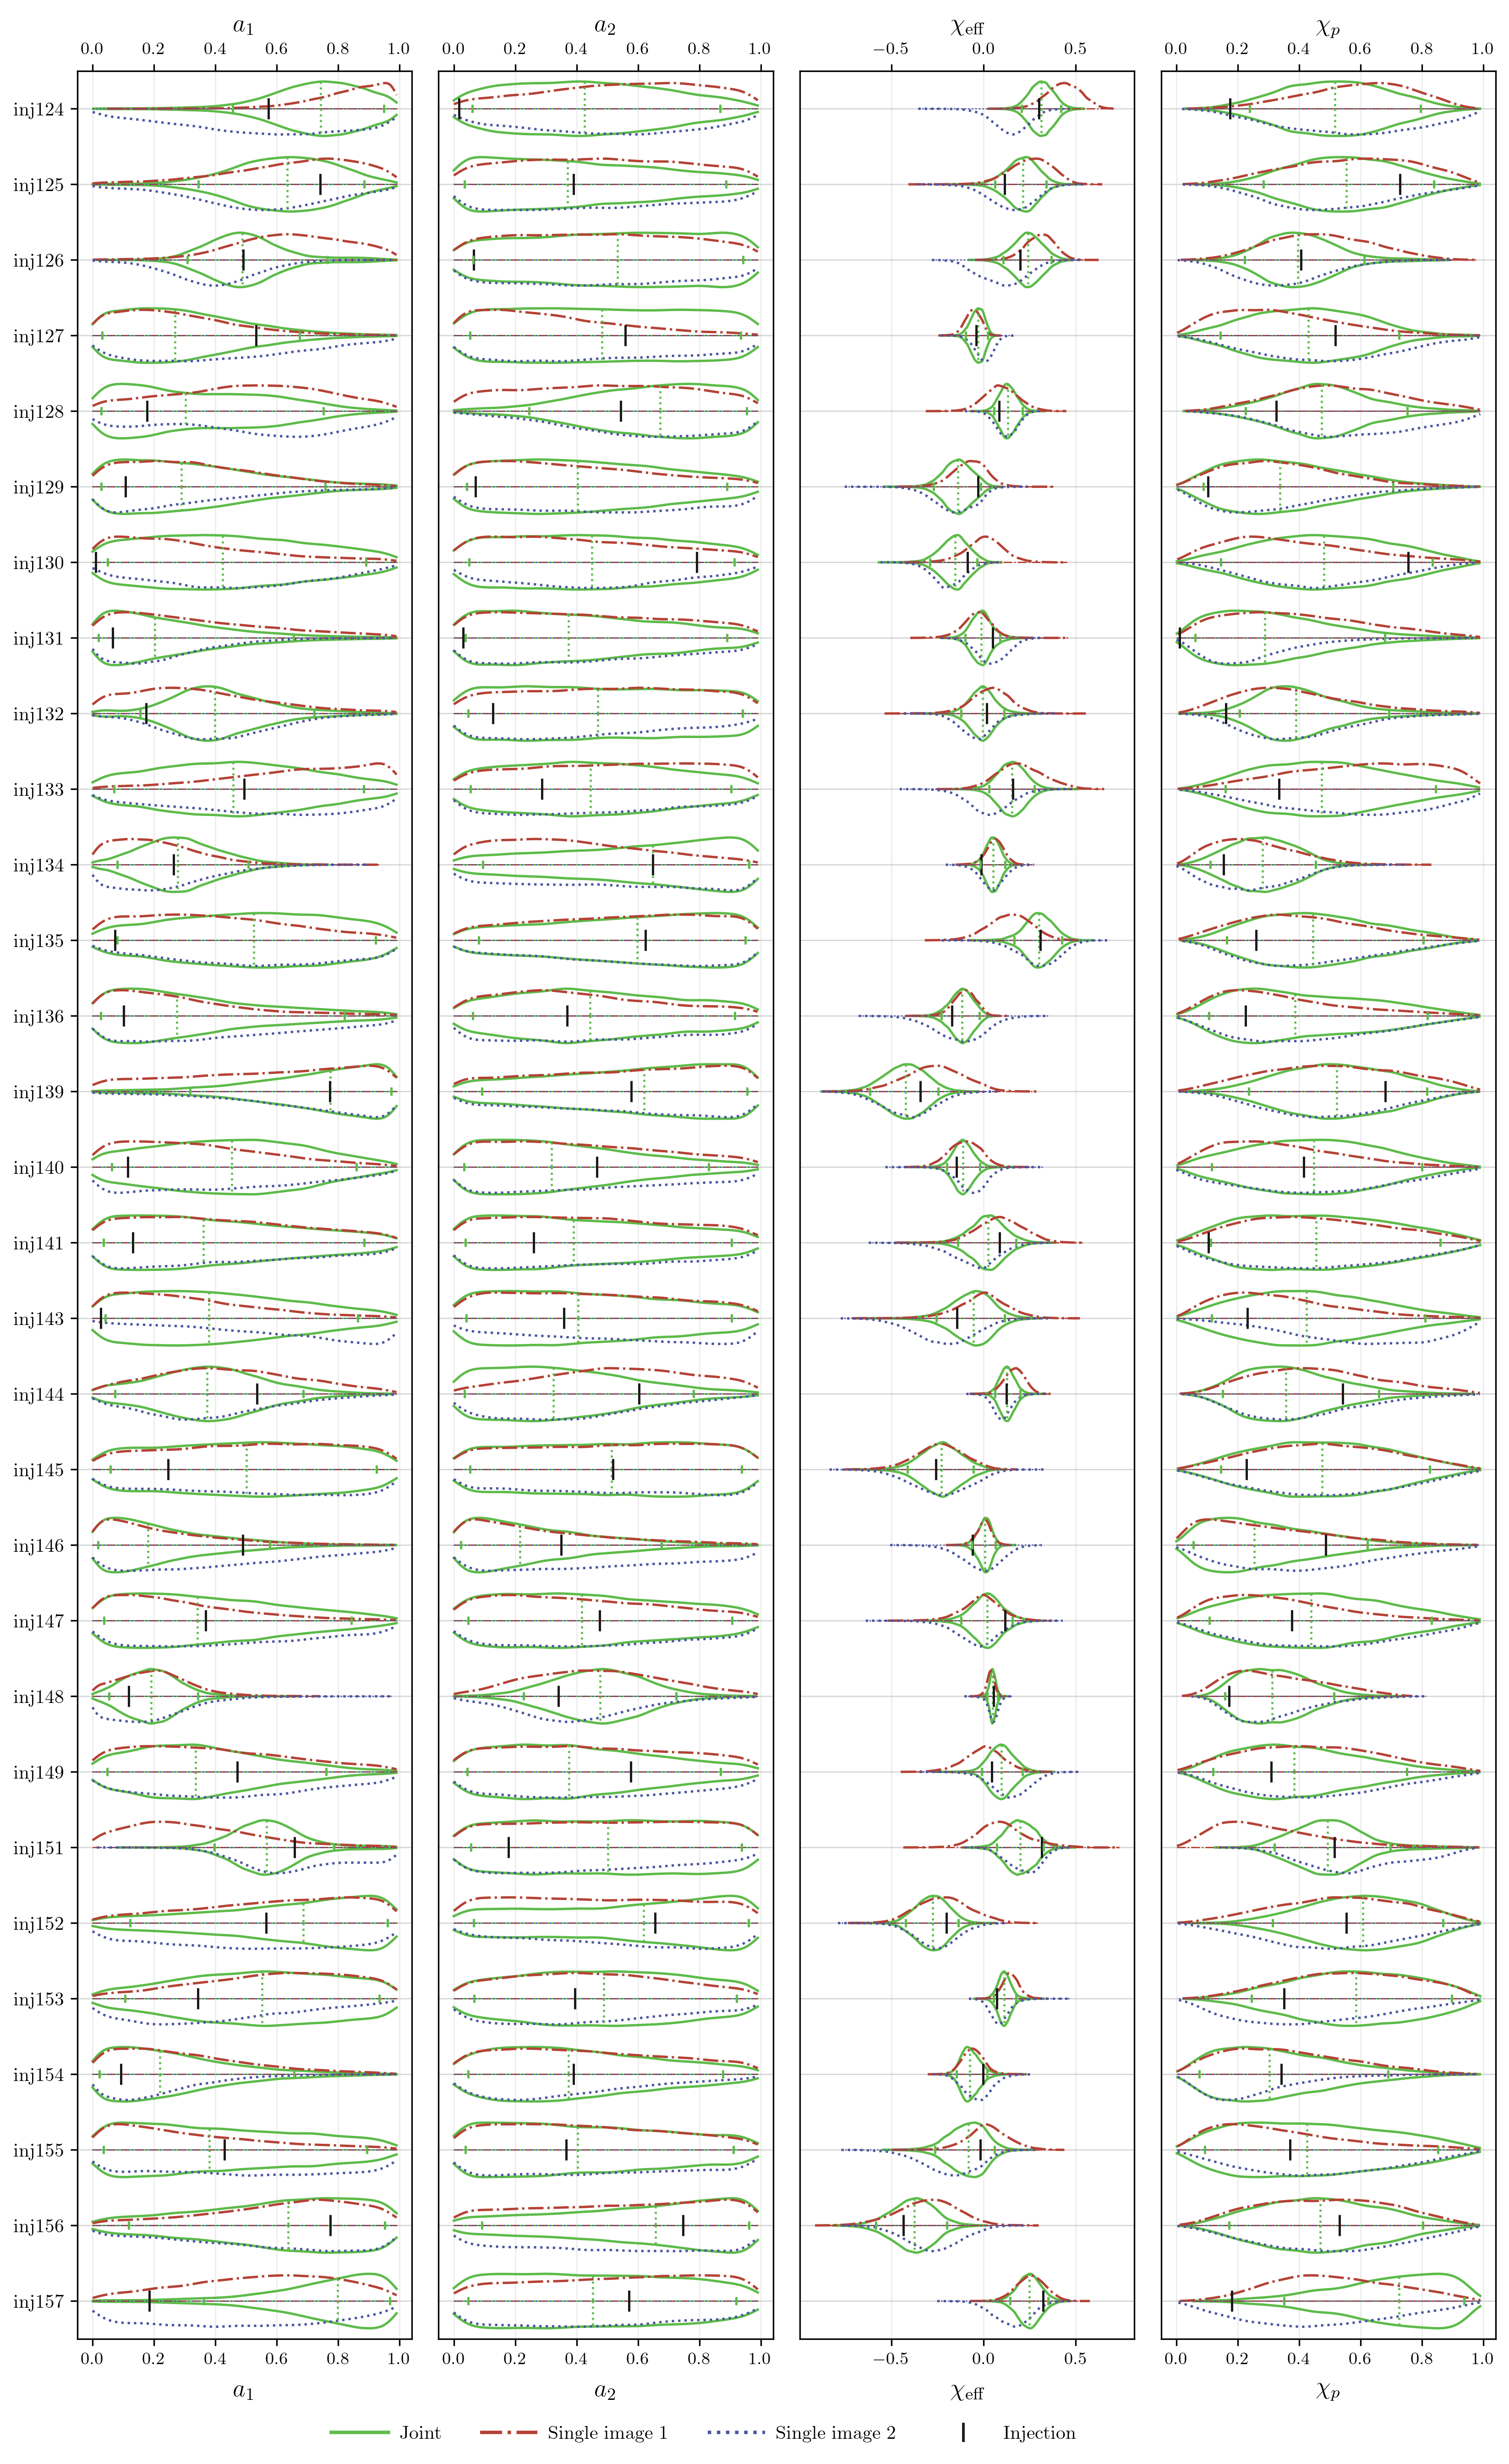
\includegraphics[height=0.92\textheight]{Figures/violin_spins_p05.png}
    \caption[]{Recovered posteriors of $a_1$, $a_2$, $\chi_\mathrm{eff}$, and $\chi_\mathrm{p}$ (5 of 5).}
\end{figure}
